\chapter{Evaluation}\label{ch:evaluation}

The theoretical analysis of the solvers provided in Chapter \ref{ch:method} shows that XPBD and PD-style solvers pursue fundamentally different approaches to 
performing implicit Euler integration on the equations of motion. XPBD employs a local Gauss-Seidel-type solver that independently minimizes energies one-by-one by 
performing corresponding constraint projections. On the other hand, PD-style solvers treat implicit integration as an 
optimization problem and attempt to minimize the objective function of the variational form of implicit Euler integration (see Sec.\ \ref{ss:variational-implicit-euler}). 
In contrast to XPBD, all PD-style solvers contain a global optimization step that enables making compromises during the minimization of multiple 
competing energies or constraints. The goal of this section is to provide experimental data that highlights how the differences between the solvers manifest themselves 
in practice during the simulation of deformable three-dimensional bodies. Starting from experiments using the simple strain material model, we extend our analysis to the more 
complex Neohookean material model and incompatible constraint sets. Here, we say that a set of constraints is incompatible if there are no particle positions 
$\vecm{q}$ that simultaneously minimize all constraints from the set.

The main tool for comparing solvers used in this report consists of setting up identical simulation states and analyzing the positions computed by the solvers during 
each of the iterations required for the simulation of a single time step. We provide a detailed description of the simulated scenarios in 
Section \ref{ss:experimental-setup} and discuss how insights on various solver properties can be gained from the positions achieved after each iteration in 
Section \ref{ss:analysis-solvers}. During our comparison of the solvers, we exclude PBD due to the fact that it is not derived from the equations of motion and does not produce 
physically accurate results (see Sec.\ \ref{ss:pbd-properties}). We provide experimental data to justify this decision in Section \ref{ss:physical-pbd}. Additionally, before a meaningful 
comparison of ADMM with other solvers is possible, suitable ADMM weights need to be determined (see Sec.\ \ref{s:admm}). We provide insights on choosing ADMM weights in Section \ref{ss:admm-weights}. 
We start our comparison between XPBD and PD-style solvers on simulations using only tetrahedral constraints for the strain material model (see Sec.\ \ref{ss:strain-material}) 
in Section \ref{ss:untwisting-beam-strain}. The effects of adding position constraints that are incompatible with the material constraints are analyzed in 
Section \ref{ss:twisting-beam-strain}. The experiments in Section \ref{ss:untwisting-beam-strain} are repeated for the simplified Neohookean material model (see 
Sec.\ \ref{ss:simplified-neohookean-material}) in Section \ref{ss:untwisting-beam-neohookean} to gain insights on the compatibility of the solvers with more complicated non-linear 
material models. Finally, we summarize our findings in Section \ref{s:discussion}.

\section{Experimental Setup}\label{ss:experimental-setup}
Experiments start from the deformed configuration of a cuboid beam that has been twisted in opposite directions at both ends (see Fig. \ref{fig:twisting-beam-setup}, left).
This initial deformed configuration is determined by simulating the twisting motion of the beam using the QN solver with a large number 
of iterations. Twisting is achieved by in-plane rotation of the reference positions 
of position constraints acting on particles at the ends of the beam. 

Starting from this configuration, we investigate the behavior of the 
solvers during the next time step in two settings: In the first, the position constraints at the ends of the beam are released, causing the 
beam to untwist (see Fig. \ref{fig:twisting-beam-setup}, top right). In the second, the beam is twisted further in accordance with a fixed angular
velocity as described above (see Fig. \ref{fig:twisting-beam-setup}, bottom right). In both settings, the initial positions of the twisted beam 
need to be updated to adapt to the changes to the position constraints at the ends of the beam. In the untwisting beam experiments, all constraints are satisfied at the 
undeformed reference configuration of the beam $\vecm{q}_\text{ref}$. However, the position constraints causing the twisting motion in the twisting beam experiments are 
incompatible with the tetrahedral constraints derived from the material model of interest. 

Position constraints are modelled via springs with rest-length zero and finite stiffness for all solvers. In other words, only soft position constraints 
are used. This has two main advantages: Firstly, soft position constraints can easily be modelled using each of the solvers, while it is challenging (or impossible) to 
implement hard position constraints with PD and QN. Mixing soft and hard position constraints makes it impossible to compare solvers,
since they would converge towards distinct solutions. Secondly, soft position constraints have corresponding spring energies that are 
finite and continuously differentiable. This allows for the computation of common metrics of deformed configurations such as the constraint 
energy. 

The elastic properties of the beam are modelled via the strain material model and the simplified Neohookean 
material model (see Sec.\ \ref{ss:material-models}). The strain model is supported by all solvers, whereas the simplified Neohookean model is 
not supported by PD. The simplified Neohookean model is chosen over the original Neohookean model because the log term in the original 
Neohookean energy potential makes it incompatible with XPBD (see Sec.\ \ref{ss:xpbd-deformable-bodies}). The experiments are run for time steps 
\SI{1e-1}{\second}, \SI{1e-2}{\second}, \SI{1e-3}{\second} and \SI{1e-4}{\second}. For the strain and Neohookean constraints, both 
stiffness and Youngs modulus, respectively, are set to powers of ten ranging from \num{1e5} to \num{1e12}. The Poisson ratio is fixed 
at 0.45 for all experiments, since we put the focus of our evalution on material stiffness over incompressibility. A representative subset of both twisting and untwisting 
beam experiments using the strain material model are discussed in Sections \ref{ss:untwisting-beam-strain} and \ref{ss:twisting-beam-strain}, respectively. For the 
Neohookean material model, we focus on the untwisting beam experiment in order to isolate the effects caused by applying solvers to a more complicated non-linear material 
model from artifacts caused by incompatible constraints. A representative set of experiments is discussed in Section \ref{ss:untwisting-beam-neohookean}.

\begin{figure}[h]
    \centering
    \begin{tikzpicture}
    \node[inner sep=0pt] (twisted) at (0,-1.625)
        {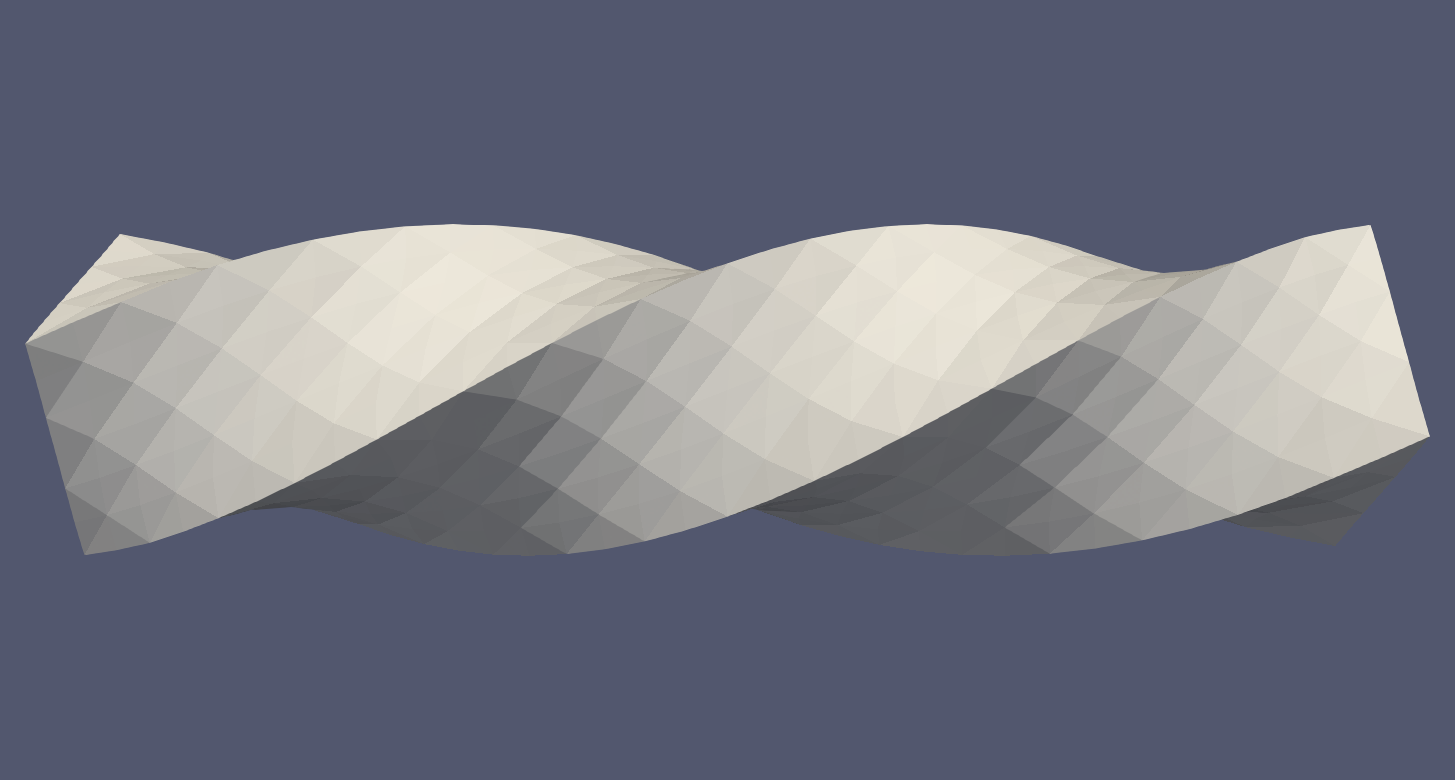
\includegraphics[width=.40\textwidth]{figures/twisted_beam.png}};
    \node[inner sep=0pt] (untwisted) at (8, 0)
        {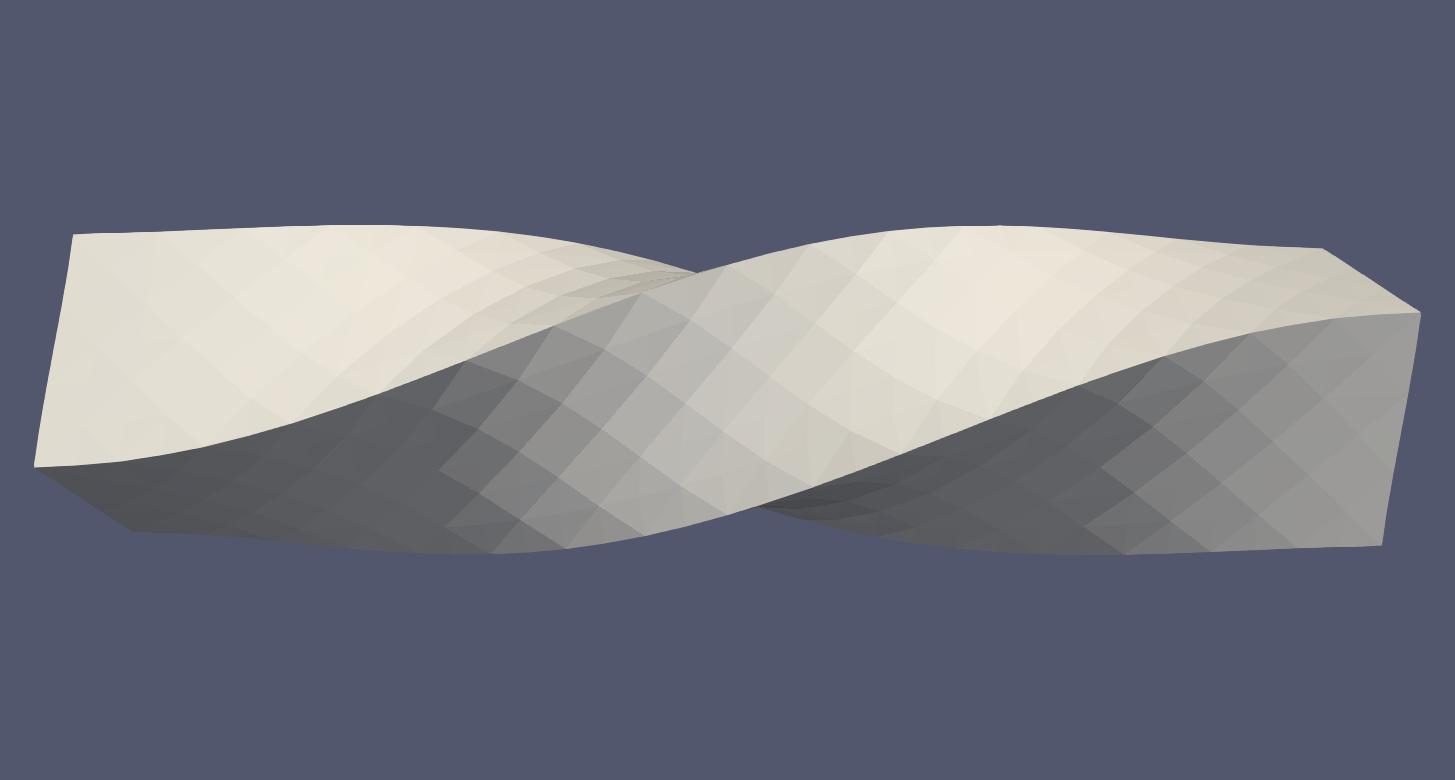
\includegraphics[width=.40\textwidth]{figures/untwisted_beam.png}};
    \node[inner sep=0pt] (further-twisted) at (8,-3.25)
        {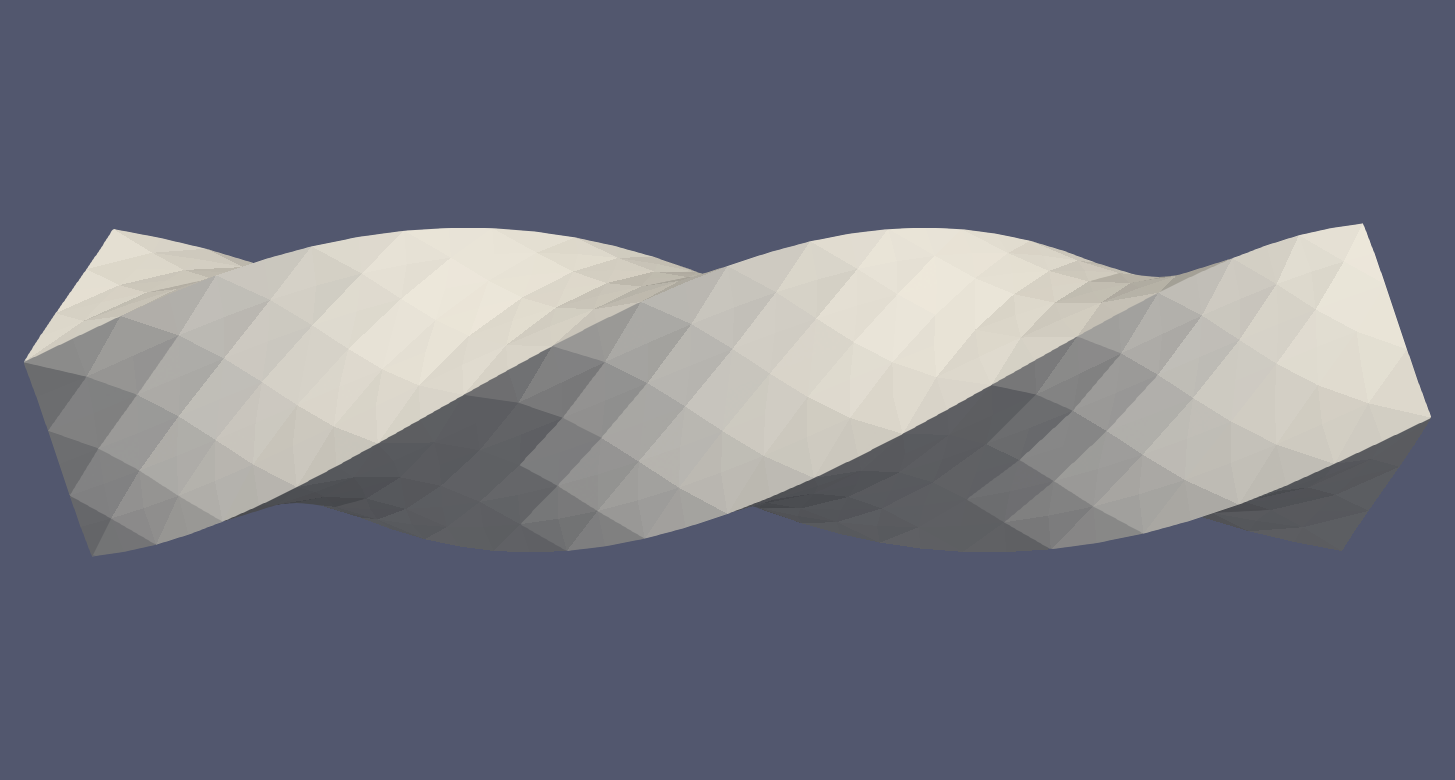
\includegraphics[width=.40\textwidth]{figures/further_twisted_beam.png}};
    \draw[->,thick] (twisted.east) -- (untwisted.west)
        node[midway,fill=white] {untwist};
    \draw[->,thick] (twisted.east) -- (further-twisted.west)
        node[midway,fill=white] {twist further};
    \end{tikzpicture}
    \caption{Visualization of the experimental settings starting from a twisted beam. The beam is either untwisted by removing position constraints at the 
    ends of the beam (top) or twisted further by rotating the anchor positions of the position constraints in-plane (bottom).}
    \label{fig:twisting-beam-setup}
\end{figure}

\section{Analyzing Solver Properties}\label{ss:analysis-solvers}
In many cases, poor solver performance is immediately obvious from closer inspection of the computed geometry. However, sometimes solvers can produce geometries 
that pass the eye test, but are in violation of the equations of motion. This is particularly applicable to small time step sizes. Thus, additional metrics are 
required to reliably evaluate solver performance across a variety of different time step sizes and stiffnesses. 

\paragraph{Objective Function of the Variational Form of Implicit Euler Integration.}
With the exception of PBD, all solvers discussed in the context of this thesis are based on implicit Euler integration of the equations of 
motion (see Sec.\ \ref{ss:numerical-integration}) and aim to either approximate (XPBD) or compute exactly (PD, ADMM and QN) the implicit positions at the next time step. 
As discussed in Section \ref{ss:numerical-integration}, the implicit positions can be interpreted as the positions that minimize the objective function of the variational 
form of implicit Euler integration given in Equation \ref{eq:variational-implicit}. To gain initial insights into the convergence behavior of the solvers, we compute 
the objective function value, or simply objective value for short, for the positions obtained after each iteration for each solver. The objective is restated here 
for the convenience of the reader

\begin{equation}\label{eq:variational-implicit-copy}
    f_{\text{obj}}(\vecm{q}) \coloneqq \min_{\vecm{q}} \frac{1}{2h^2} \norm{\matm{M}^{\frac{1}{2}}(\vecm{q} - \tilde{\vecm{q}})}^2_F + \sum_j \psi_j(\vecm{q}).
\end{equation}

\noindent The solvers are expected to decrease the objective with each iteration until a value close to the minimum obtained 
by the implicit positions is achieved. By comparing the objective values after the final iteration, the quality of the configurations different
solvers converge to can be analyzed. Further, by plotting the objective values over the iteration number and inspecting the slope of the graphs, information about
the convergence rates of the solvers can be inferred. During the discussion of the resulting figures, we consider a solver converged once the graph of its objective function 
value over the iterations is visually indistinguishable from a horizontal line. While not entirely rigorous, this is particularly appropriate for comparing solvers in the 
context of real-time applications where solver iterations that only make minor progress towards the true implicit solutions often cannot be afforded. Additionally, this 
allows setting the focus on the most important qualitative differences between solvers without getting lost in the details of when a solver can formally be considered converged.

As discussed in Section \ref{ss:variational-implicit-euler}, the constraint term of the objective function corresponds to the sum of the constraint energies, while the 
inertial term introduces a penalty for moving particles away from their inertial positions $\tilde{\vecm{q}}$. However, in the context of the untwisting and twisting beam 
experiments described in Section \ref{ss:experimental-setup}, the inertial term can also be interpreted as the kinetic energy of the beam. To see this, note that both the initial 
particle velocities $\vecm{v}_0$ and the external forces $\vecm{f}_{\text{ext}}$ acting on the simulated body are zero. Consequently, the inertial positions $\tilde{\vecm{q}}$ 
are equivalent to the initial positions $\vecm{q}_0$, as shown below

\[ 
    \tilde{\vecm{q}} = \vecm{q}_0 + h\vecm{v}_0 + h^2\matm{M}^{-1}\vecm{f}_{\text{ext}} = \vecm{q}_0.
\]

\noindent It follows that the inertial term at the positions achieved after $k$ solver iterations $\vecm{q}_k$ can be rewritten as

\[
    \frac{1}{2h^2} \norm{\matm{M}^{\frac{1}{2}}(\vecm{q}_k - \vecm{q}_0)}^2_F 
    = \frac{1}{2} \norm{\matm{M}^{\frac{1}{2}}\frac{\vecm{q}_k - \vecm{q}_0}{h}}^2_F
    = \frac{1}{2} \norm{\matm{M}^{\frac{1}{2}}\vecm{v}_k}^2_F,
\]

\noindent where $\vecm{v}_k$ are the particle velocities after $k$ iterations as computed via Verlet integration. The last term in the equation above is exactly the 
kinetic energy of the simulated body. As the sum of the elastic and kinetic energy, the objective function can be interpreted as the energy of the beam. According 
to Newton's laws, this energy should be conserved in the absence of external forces. However, implicit Euler integration typically introduces numerical 
damping which is expected to reduce the energy of the beam over time (see Sec.\ \ref{ss:numerical-integration}).

\paragraph{Linear and Angular Momentum.}
Since adding artificial linear and angular momentum to simulations manifests itself in ghost forces which act like external forces dragging and rotating the object, 
conserving global momenta is a hard requirement for achieving visually plausible simulations \cite{mueller2006}. If the elastic forces in the equations of motion are 
derived from rigid motion invariant energy potentials, the true positions resulting from implicit Euler integration 
conserve linear and angular momentum \cite{bouaziz2014}. However, there are many situations where we cannot expect solvers to converge to the true implicit positions. 
As an example, we have shown that XPBD cannot be said to solve the equations of motions exactly due to simplifying assumptions made during the derivation of the XPBD 
constraint projection (see Sec.\ \ref{ss:xpbd-properties}). Additionally, in the context of real-time applications, the number of solver iterations is often fixed to ensure 
that the physics simulation fits into the allotted time budget. In such situations, there is no guarantee that solvers converge in the available number of iterations. 
Thus, it is important to analyze whether solvers conserve global momenta at both the converged configuration and the intermediate configurations achieved after each 
solver iteration. The computation of the linear and angular momentum after solver iteration $k$ requires the computation of velocities $\vecm{v}_k$ from the current 
positions $\vecm{q}_k$. In our experiments, we compute velocities $\vecm{v}_k$ by performing a Verlet integration step given by

\begin{equation}\label{eq:velocities}
    \vecm{v}_k = \frac{\vecm{q}_k - \vecm{q}_0}{h},
\end{equation}

\noindent where $h$ is the time step size. Now, let $i$ denote a particle index and let $\vecm{q}$ and $\vecm{v}$ denote the current particle positions and velocities, 
respectively. Then, the global linear momentum is equal to 

\begin{equation}\label{eq:linear-momentum}
    \sum_i m_i \vecm{v}_i,
\end{equation}

\noindent and the angular momentum with respect to some point $\vecm{p} \in $ is given by 

\begin{equation}\label{eq:angular_momentum}
    \sum_i (\vecm{q}_i - \vecm{p}) \times (m_i \vecm{v}_i).
\end{equation}

\section{Physically-Based PBD}\label{ss:physical-pbd}
In contrast to XPBD and the PD-style solvers, PBD is not derived from the implicit integration of the equations of motion. As a result, the stiffness of materials 
simulated using PBD depends on the number of iterations and the chosen time step (see Sec.\ \ref{ss:pbd-properties}). Accordingly, in the limit of infinite iterations and zero 
time step size, the material becomes infinitely stiff. We demonstrate this effect by example of a single solve over time steps \SI{1e-2}{\second} and \SI{1e-3}{\second} in the 
untwisting beam setting (see Fig. \ref{fig:twisting-beam-setup}) using strain constraints with stiffness \num{1e8} in Figure \ref{fig:strain-pbd}. The experiment shows that the 
beam is untwisted entirely to its undeformed reference configuration when using the PBD solver, regardless of the chosen time step. On the other hand, the degree to which the 
beam is untwisted depends on the time step size when using the QN solver. In particular, the beam untwists further when the larger time step of \SI{1e-2}{\second} 
is used. Of course, the behavior of the PBD solver is not physically plausible. This observation and the fact that PBD can seamlessly be extended to XPBD at the cost of storing 
a single additional variable per constraint leads us to the decision to exclude PBD from the remaining experiments in this thesis and to focus on analyzing the properties of 
XPBD, ADMM, PD and the QN solver instead.

\begin{figure}
    \begin{subfigure}{0.49\textwidth}
    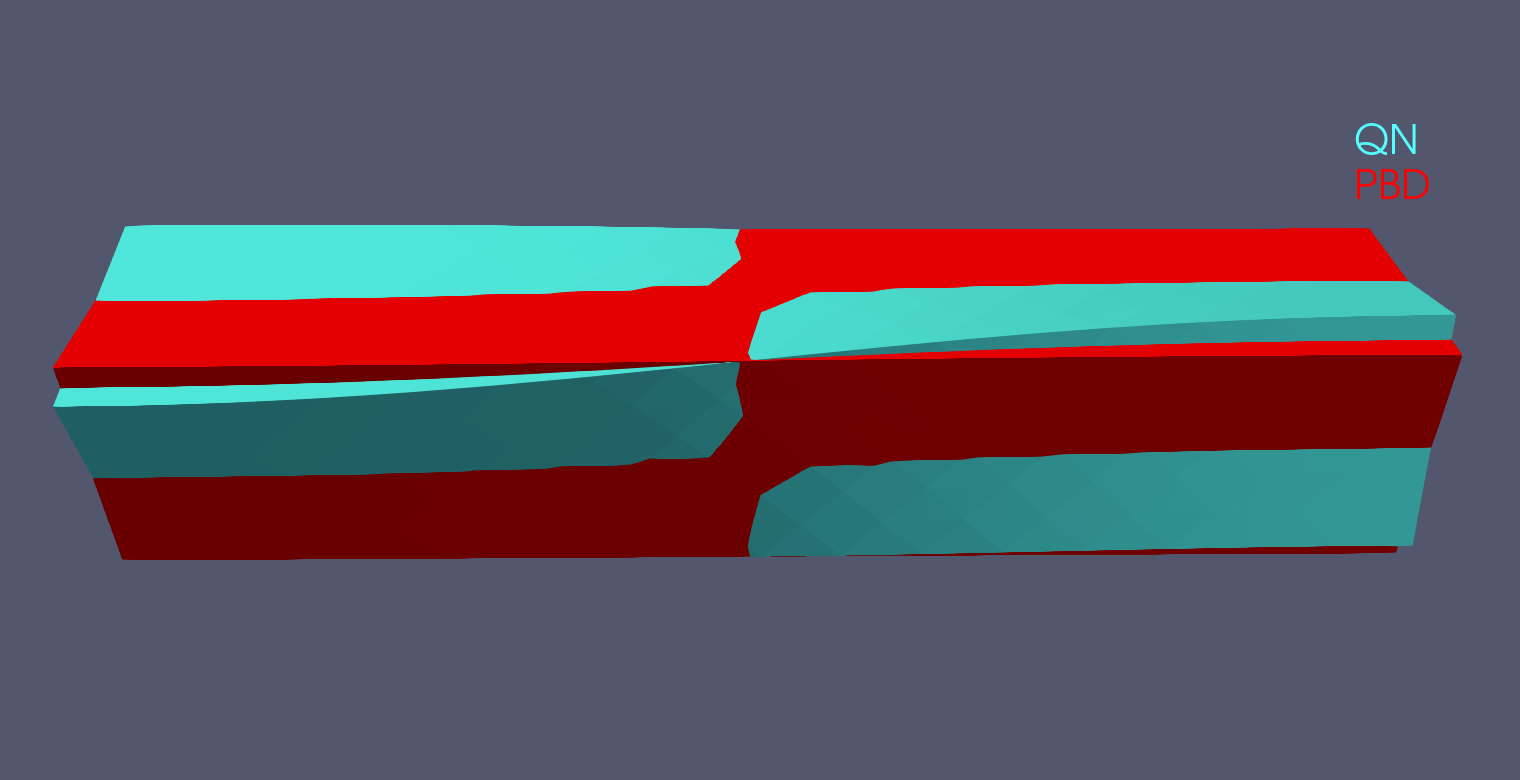
\includegraphics[width=\textwidth, trim={0 5.0cm 0 2.5cm}, clip]{figures/strain_pbd_1e-2.png}
    \subcaption{time step \SI{1e-2}{\second}}
    \end{subfigure}
    \begin{subfigure}{0.49\textwidth}
    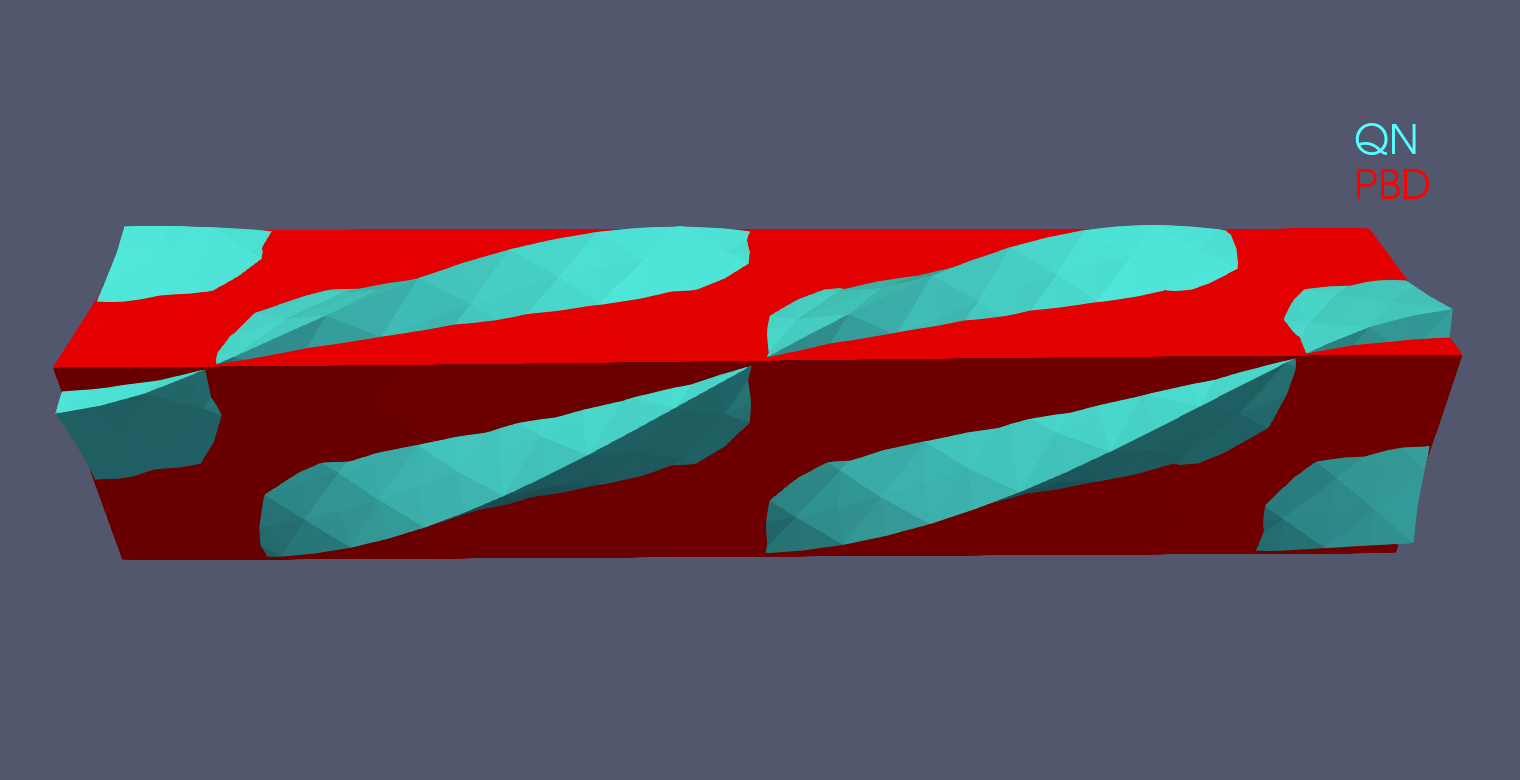
\includegraphics[width=\textwidth, trim={0 5.0cm 0 2.5cm}, clip]{figures/strain_pbd_1e-3.png}
    \subcaption{time step \SI{1e-3}{\second}}
    \end{subfigure}
    \caption{Geometries of an untwisting beam with strain constraints (stiffness \num{1e8}) after 1000 iterations over a single time step of size \SI{1e-2}{\second} (left) 
    and \SI{1e-3}{\second} (right) using PBD (red) and QN (cyan).}
    \label{fig:strain-pbd}
\end{figure}


\section{ADMM Weights}\label{ss:admm-weights}
As stated in Section \ref{ss:admm-properties}, there is no generally valid method for determining ADMM weights that ensures acceptable convergence properties.
Thus, we need to manually fine-tune ADMM weights before comparing different solvers using the method described above. The convergence of the ADMM solver is evaluated via 
the objective function of the beam (see Sec.\ \ref{ss:analysis-solvers}). We focus on untwisting beam experiments using strain constraints. For 
each combination of time steps from \SI{1e-1} to \SI{1e-4} and stiffnesses $k$ from \num{1e5} to \num{1e12}, candidate weights around the recommended value $w_i = \sqrt{k}$ 
are generated and the weight that reduces the objective function the fastest is used as the ADMM weight for all following experiments. 
This process reveals that ADMM weights are in fact time step dependent.

To see this, consider the plots of the objective values over the number of ADMM iterations with different weights for time steps \SI{1e-2}{\second} and 
\SI{1e-3}{\second} with constraint stiffness \num{1e8} shown in Figure \ref{fig:strain-weights-admm}. When a time step 
of \SI{1e-2}{\second} is used (see Fig. \ref{fig:strain-weights-admm} a), the ADMM solver converges to the same objective value for all of the weights, except for the 
lowest weight $w_i = 0.1\sqrt{k}$, where the value is increased compared to the initial objective value. The fastest convergence is achieved by setting $w_i = 0.3\sqrt{k}$ and 
$w_i = 0.4\sqrt{k}$. When picking smaller weights, the objective value is larger than the initial objective value during the first 20 iterations. Setting the weights to 
higher values than $w_i = 0.4\sqrt{k}$ leads to a slower convergence rate. However, if the time step is decreased to \SI{1e-3}{\second} (see Fig. \ref{fig:strain-weights-admm} b), 
weights higher than $w_i = 0.4\sqrt{k}$ achieve a better convergence rate and converge to configurations with a lower objective value than weights lower than 
or equal to $w_i = 0.4\sqrt{k}$. In particular, ADMM converges to a solution whose objective value is higher than the initial objective value when using $w_i = 0.2\sqrt{k}$ and 
$w_i = 0.3\sqrt{k}$. Thus, $w_i = 0.3\sqrt{k}$ is an excellent weight for time step \SI{1e-2}{\second}, while it is unsuitable for time step \SI{1e-3}{\second}. Overall, it 
can be seen that more aggressive reductions of the ADMM weights without jeopardizing convergence are possible when a larger time step is used. Qualitatively equivalent results 
can be observed for other stiffness values. 

In Section \ref{ss:admm-properties}, we hypothesized that it might be preferrable to use smaller ADMM weights if the constraint energy $\Psi$ is significantly smaller at the true 
implicit positions $\vecm{q}^*$ than at the initial positions $\vecm{q}_0$, whereas larger weights might be more appropriate when $\Psi(\vecm{q}^*) \approx \Psi(\vecm{q}_0)$.
The time step dependence of ADMM weights can be explained by combining this insight with the fact that the extent to which a single application of implicit Euler integration 
reduces the constraint energy of a deformed body generally grows with increasing time step size. Thus, for smaller time steps it is 
$\Psi(\vecm{q}^*) \approx \Psi(\vecm{q}_0)$, favoring the use of larger ADMM weights. Note that this time step dependence 
makes finding suitable ADMM weights incredibly tedious: For each material model, weights need to be manually fine-tuned for each combination of time step size and 
material stiffness. To save time, we reuse the ADMM weights determined for the untwisting beam experiments (see Sec.\ \ref{ss:untwisting-beam-strain}) in the twisting 
beam experiments (see Sec.\ \ref{ss:twisting-beam-strain}). However, it is not clear whether ADMM weights can be reused across different simulation scenarios, even if the time step 
size and the material stiffness remain unchanged.

\begin{figure}[h]
    \centering
    \begin{subfigure}{\textwidth}
        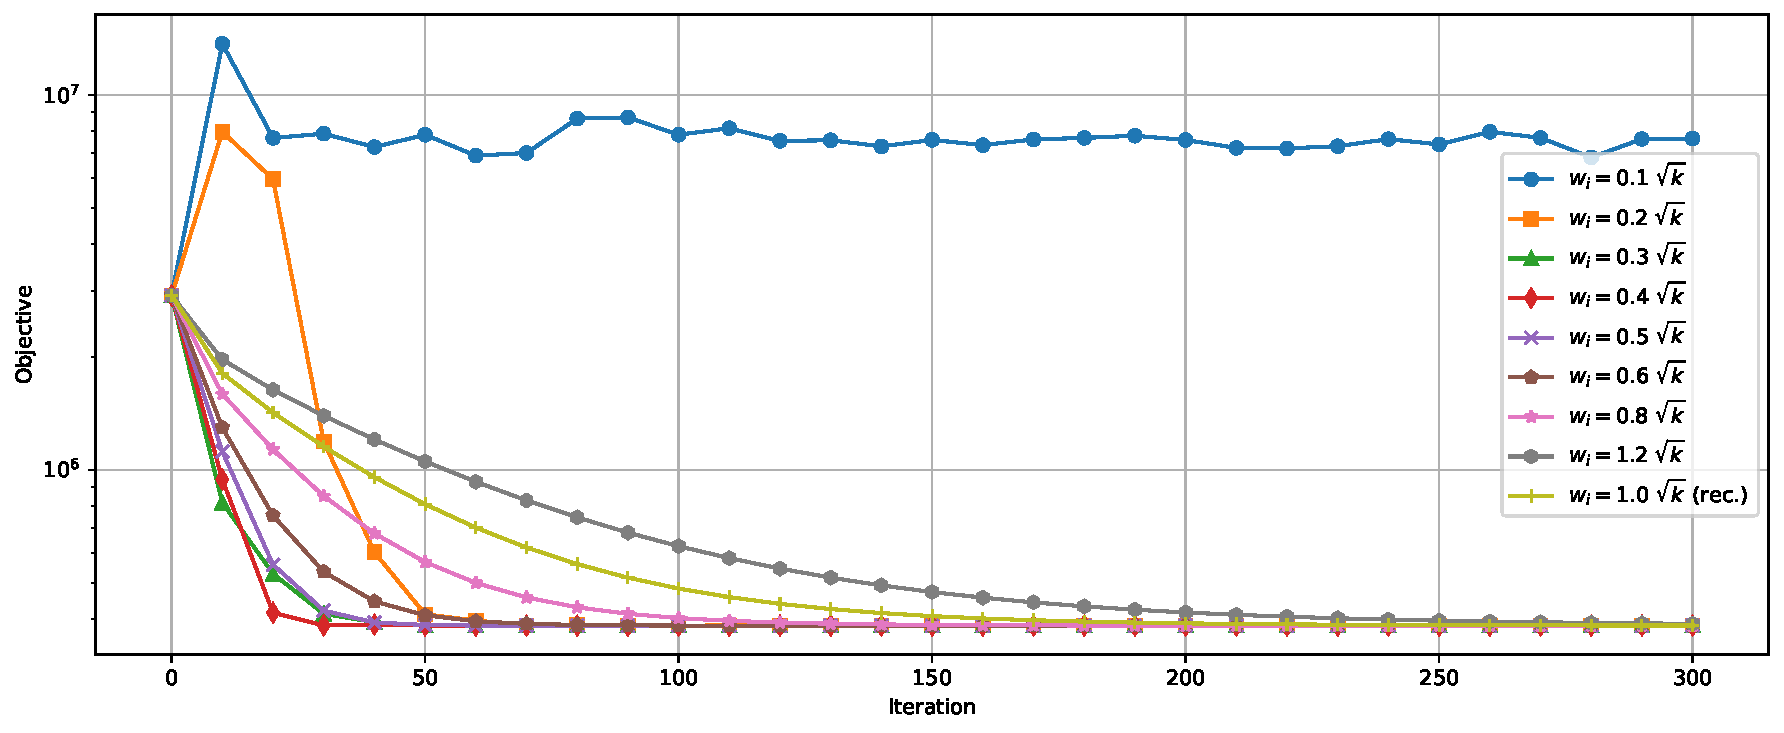
\includegraphics[width=\linewidth]{figures/strain_admm_weights_1e-2.pdf}
        \subcaption{Time step \SI{1e-2}{\second}}
    \end{subfigure}
    \begin{subfigure}{\textwidth}
        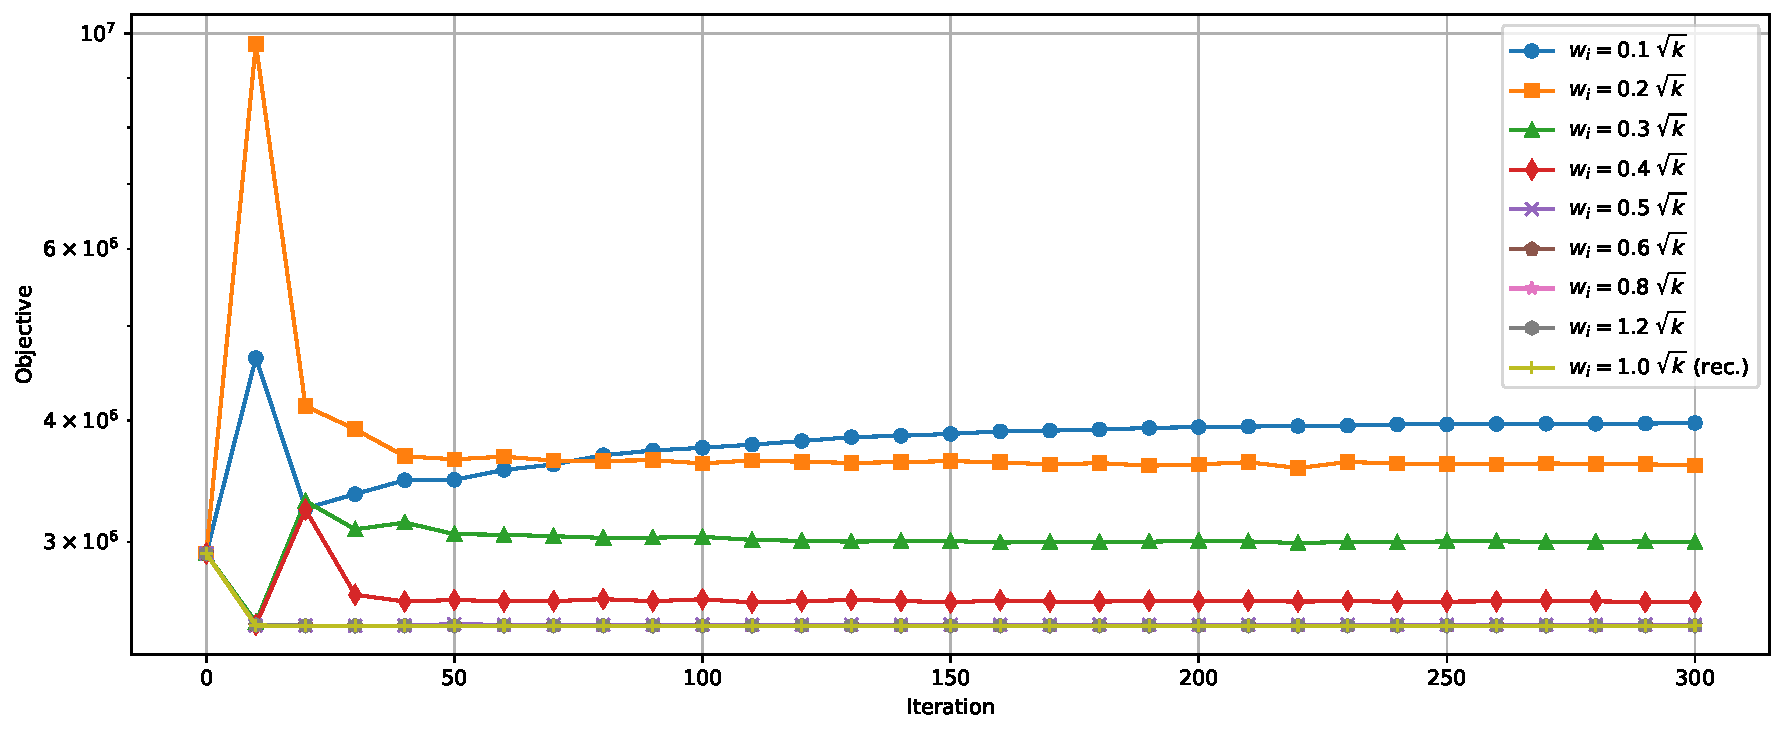
\includegraphics[width=\linewidth]{figures/strain_admm_weights_1e-3.pdf}
        \subcaption{Time step \SI{1e-3}{\second}}
    \end{subfigure}
    \caption{Values of the objective function of the variational form of implicit Euler integration (see Eq.\ \ref{eq:variational-implicit}) over the iterations of a single time 
        step of size \SI{1e-2}{\second} (a) and \SI{1e-3}{\second} (b) for an untwisting beam with strain constraints with stiffness \num{1e8} using ADMM with different weights.}
    \label{fig:strain-weights-admm}
\end{figure}

\section{Untwisting Beam Simulations - Strain Material}\label{ss:untwisting-beam-strain}
In the untwisting beam experiments using the strain material model, challenges due to incompatible constraint sets are avoided and the tetrahedral strain constraints are 
easy to minimize due to the fact that corresponding restorative elastic forces are proportional to the distance between the deformation and its closest rigid-body 
transform (see Sec.\ \ref{ss:strain-material}). Thus, we use them as a starting point for highlighting differences between the different solvers. We start by comparing the 
convergence properties of different solvers in Section \ref{ss:untwisting-beam-strain-convergence}. Experimental data that suggests that solvers 
convert elastic energy stored in the deformed beam into kinetic energy is provided in Section \ref{ss:conversion-constraint-kinetic}. The effects of terminating different 
solvers after a fixed number of solver iterations are analyzed in Section \ref{ss:early-termination}. In Section \ref{ss:computational-cost-strain}, the computational costs 
of the solvers are compared. Finally, we investigate the behavior of the solvers when larger time step sizes and stiffness values are used in Sections 
\ref{ss:untwisting-beam-strain-convergence-large-ts} and \ref{ss:momenta-large-ts}.

\subsection{Convergence Properties}\label{ss:untwisting-beam-strain-convergence}
We start by analyzing the convergence properties of different solvers with time step size \SI{1e2}{\second} and stiffness \num{1e8} by plotting the objective values over the 
iteration number in Figure \ref{fig:strain-beam-untwist-objectives}. Note that the results are representative for a large range of time step sizes and stiffness 
values. The graph shows that each of the solvers indeed mostly decreases the objective from iteration to iteration until it converges towards a final configuration 
after a sufficient number of iterations. ADMM, PD and QN converge to configurations with roughly the same objective value whereas the objective value obtained after 1000 
XPBD iterations is still slightly larger. QN and ADMM converge after roughly 40 and 60 iterations, whereas PD and XPBD converge after upwards of 260 and 1000 iterations, 
respectively. To quantify the progress that other solvers achieve during the number of iterations it takes each of the solvers to converge, we compute relative errors after 
40 (QN), 60 (ADMM), 260 (PD) and 1000 (XPBD) iterations. The relative error is given by 

\begin{equation}\label{eq:rel-error}
    \frac{f_{\text{obj}}(\vecm{q}_k) - f_{\text{obj}}(\vecm{q}^*)}{f_{\text{obj}}(\vecm{q}_0) - f_{\text{obj}}(\vecm{q}^*)},
\end{equation}

\noindent where $\vecm{q}_k$ are the positions after iteration $k$ and $\vecm{q}^*$ are the positions with minimal objective value
achieved by any of the solvers. The relative errors are shown in Figure \ref{fig:rel-errors}. Note that the relative error of ADMM is only 
0.4 \% by the time QN has converged, while the errors achieved by PD and XPBD are still substantial. Additionally, even after a 1000 iterations, XPBD's relative error 
is still at 1.8 \%.

\begin{table}[h]
\centering
\begin{tabular}{ |r||c|c|c|c| } 
 \hline
 & QN & ADMM & PD & XPBD\\
 \hline
 \hline
    40 iterations (QN) & 0.0 & 0.4 & 22.7 & 67.8 \\ 
    60 iterations (ADMM) & 0.0 & 0.0 & 12.6 & 47.8 \\
    260 iterations (PD) & 0.0 & 0.0 & 0.0 & 4.0 \\
    1000 iterations (XPBD) & 0.0 & 0.0 & 0.0 & 1.8 \\ 
 \hline
\end{tabular}
\caption{Relative errors (see Eq.\ \ref{eq:rel-error}) in \% achieved by solvers after 40, 60, 260 and 1000 iterations for the untwisting beam experiment from 
Figure \ref{fig:strain-beam-untwist-objectives}.}
\label{fig:rel-errors}
\end{table}

The data suggests that ADMM, PD and QN converge towards a solution that is closer to the true implicit positions at the next time step than XPBD. This is expected, 
as XPBD only approximates a solution to the implicit equations of motion due to the simplifying assumptions made during its derivation (see Sec.\ \ref{ss:xpbd-properties}).
Due to the second assumption (see Eq.\ \ref{eq:xpbd-assumption-2}) in particular, there is no penalty for moving vertex positions away from their inertial positions during 
the XPBD constraint projections (see Sec.\ \ref{ss:xpbd-properties}), even though it increases the objective function. Additionally,
it is not clear whether the Gauss-Seidel solver at the core of XPBD is able to minimize the constraint energies sufficiently via local constraint projections only.
Since constraints are projected independently one-by-one, later constraint projections can undo some of the work achieved by previous projections. Bouaziz et al.\ 
\cite{bouaziz2014} describe this phenomenon as an oscillation between different constraints. On the other hand ADMM, PD and QN aim to solve the implicit equations 
of motion exactly. The difference in the rate of convergence between ADMM and PD goes in line 
with experimental data provided by Overby et al.\ \cite{overby2017}. There, the authors show that ADMM with a weight of $\sqrt{k}$, where $k$ is the stiffness of the 
strain constraints, is almost equivalent to PD and that the convergence rate can often be improved by reducing the weight. As discussed in 
Section \ref{ss:admm-properties}, this is due to the fact that lower weights allow faster progress towards positions that reduce the constraint energy, which is particularly 
useful for simulations with larger timesteps. Similarly, the faster convergence rate of QN compared to PD is expected in light of the observation that PD is a quasi-Newton method 
with constant Hessian approximation (see \cite{liu2017}, Sec.\ \ref{ss:pd-quasi-newton}). The QN solver augments the PD solver with a line-search algorithm and LBFGS-updates to 
the constant Hessian approximation from PD that take into account curvature information from previous iterations to better approximate the true Hessian matrix. Both
of these measures help improve the convergence rate of QN in comparison to PD. Again, this is in line with results presented by Liu et al.\ \cite{liu2017}. The comparably
slow convergence rate of XPBD could again be explained by the simplifying assumptions made during the XPBD derivation and the aforementioned oscillations of Gauss-Seidel
solvers. 

\begin{figure}[h]
    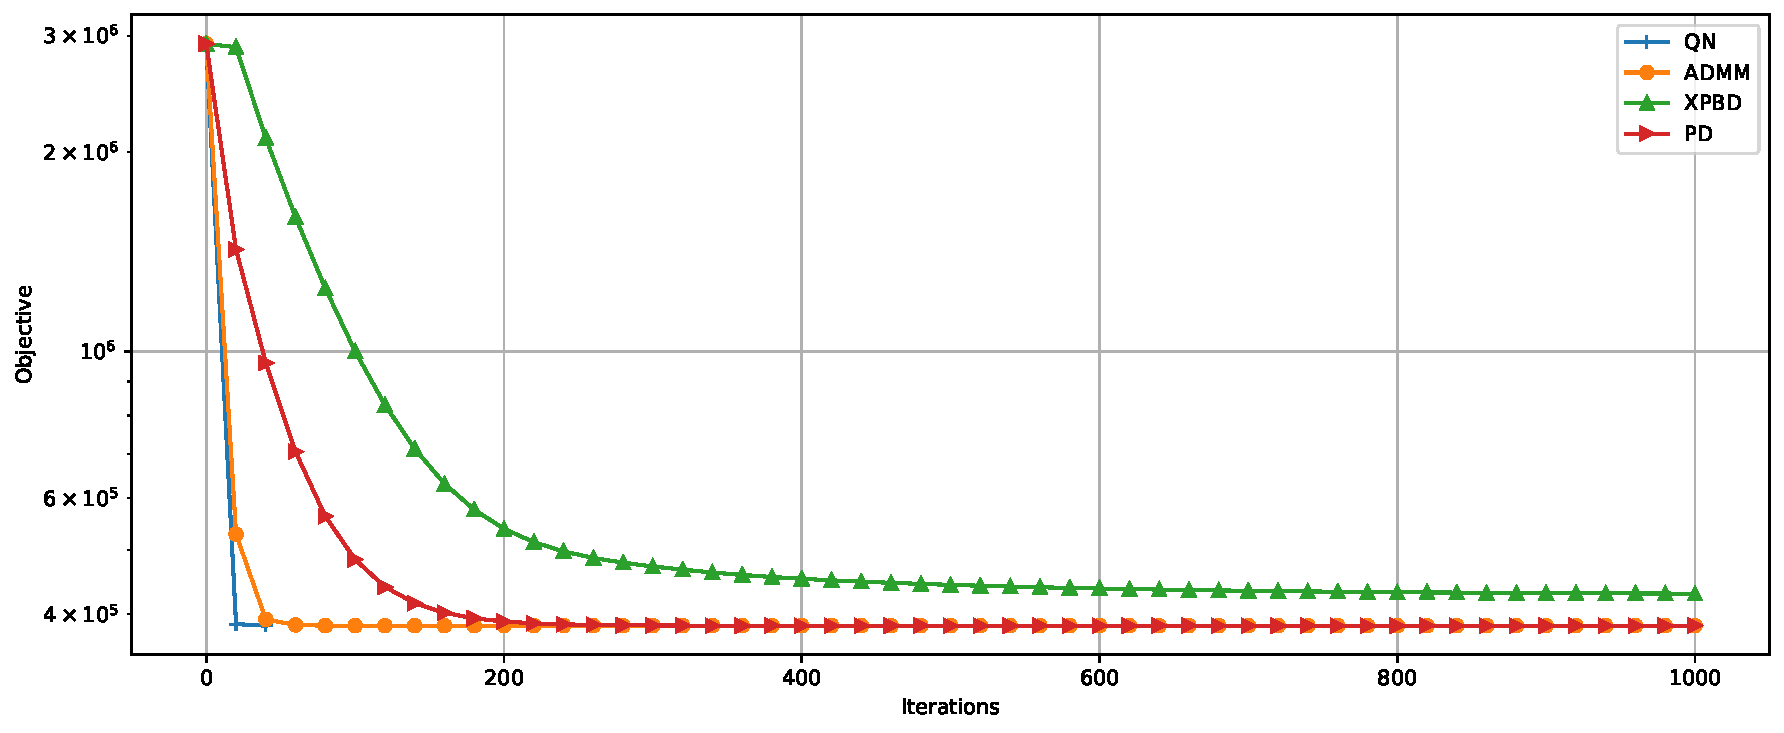
\includegraphics[width=\textwidth]{figures/strain_beam_untwist_objectives.pdf}
    \caption{Values of the objective function of the variational form of implicit Euler integration (see Eq.\ \ref{eq:variational-implicit}) over the iterations of a single time 
        step of size \SI{1e-2}{\second} for an untwisting beam using strain constraints with stiffness \num{1e8}.}
    \label{fig:strain-beam-untwist-objectives}
\end{figure}


To better understand the main factor for XPBD's unfavorable convergence properties, it is helpful to plot the inertial term and the constraint term of the objective 
function separately. The resulting plots are shown in Figure \ref{fig:strain-beam-untwist-objectives-split}. 
We focus on the first 500 iterations to gain clearer insights into the behavior of the solver during earlier iterations, since these are more relevant for 
real-time applications. First, it is evident that the constraint energy dominates the objective value for each solver during most of the iterations before 
convergence is achieved. While each solver mostly decreases the constraint energy with an increasing number of iterations, the inertial term is mostly increased. 
The only exception is the ADMM solver between iterations 30 to 60, where the inertial term is decreased from its peak and the constraint energy is increased from its 
low point. ADMM, PD and QN converge to configurations with roughly the same inertial and constraint terms. However, at its final state, the constraint 
energy of the XPBD solver is higher than its counterparts from the PD-style solvers, whereas the opposite is observed for the inertial term. 

\begin{figure}[h]
    \centering
    \begin{subfigure}{\textwidth}
        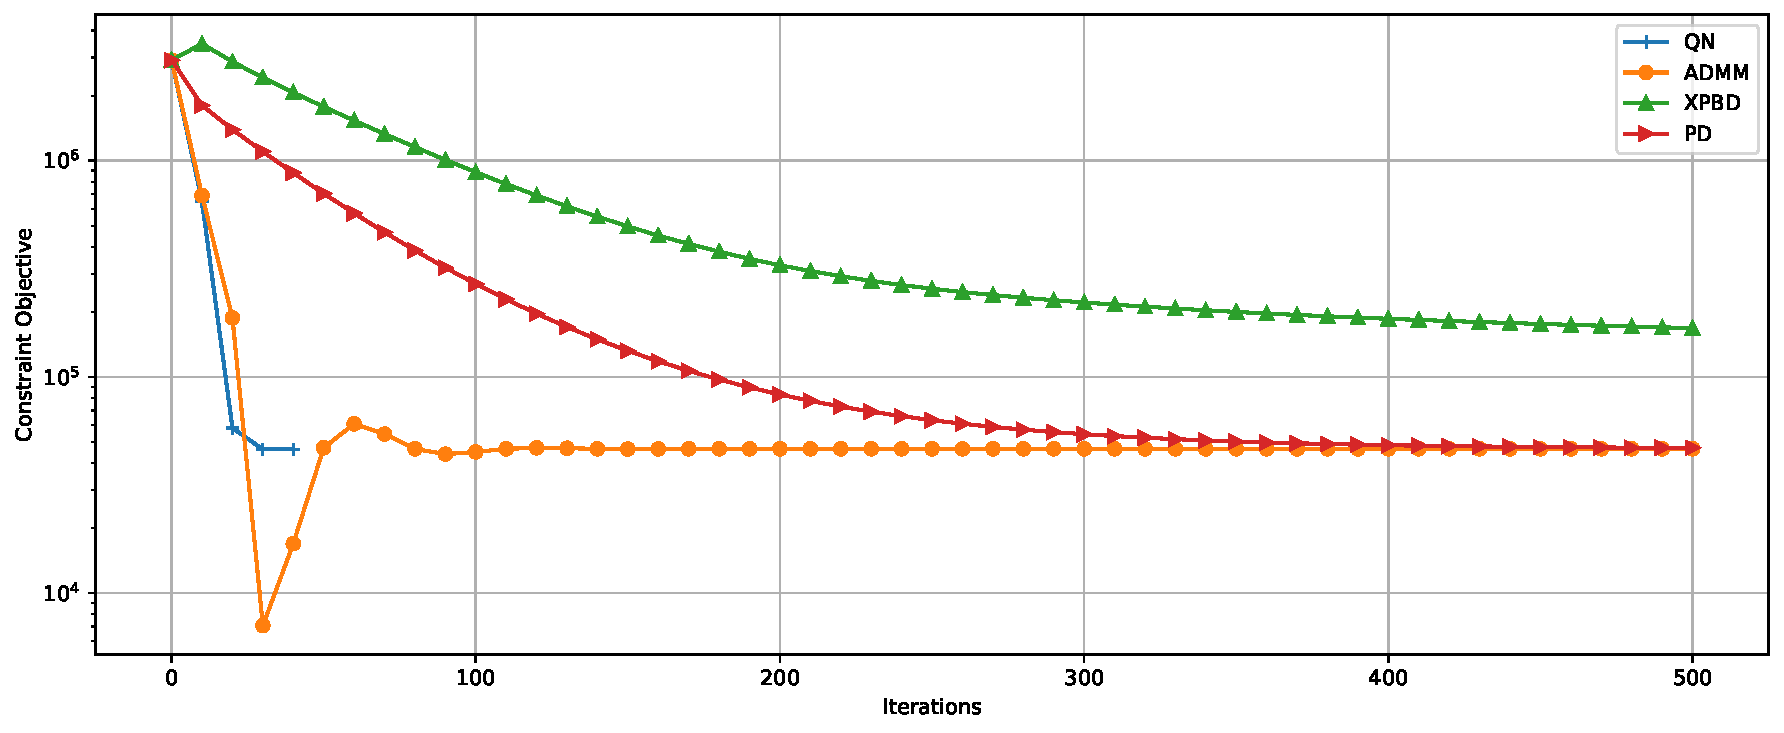
\includegraphics[width=\linewidth]{figures/strain_beam_untwist_constraintObjectives.pdf}
    \end{subfigure}
    \begin{subfigure}{\textwidth}
        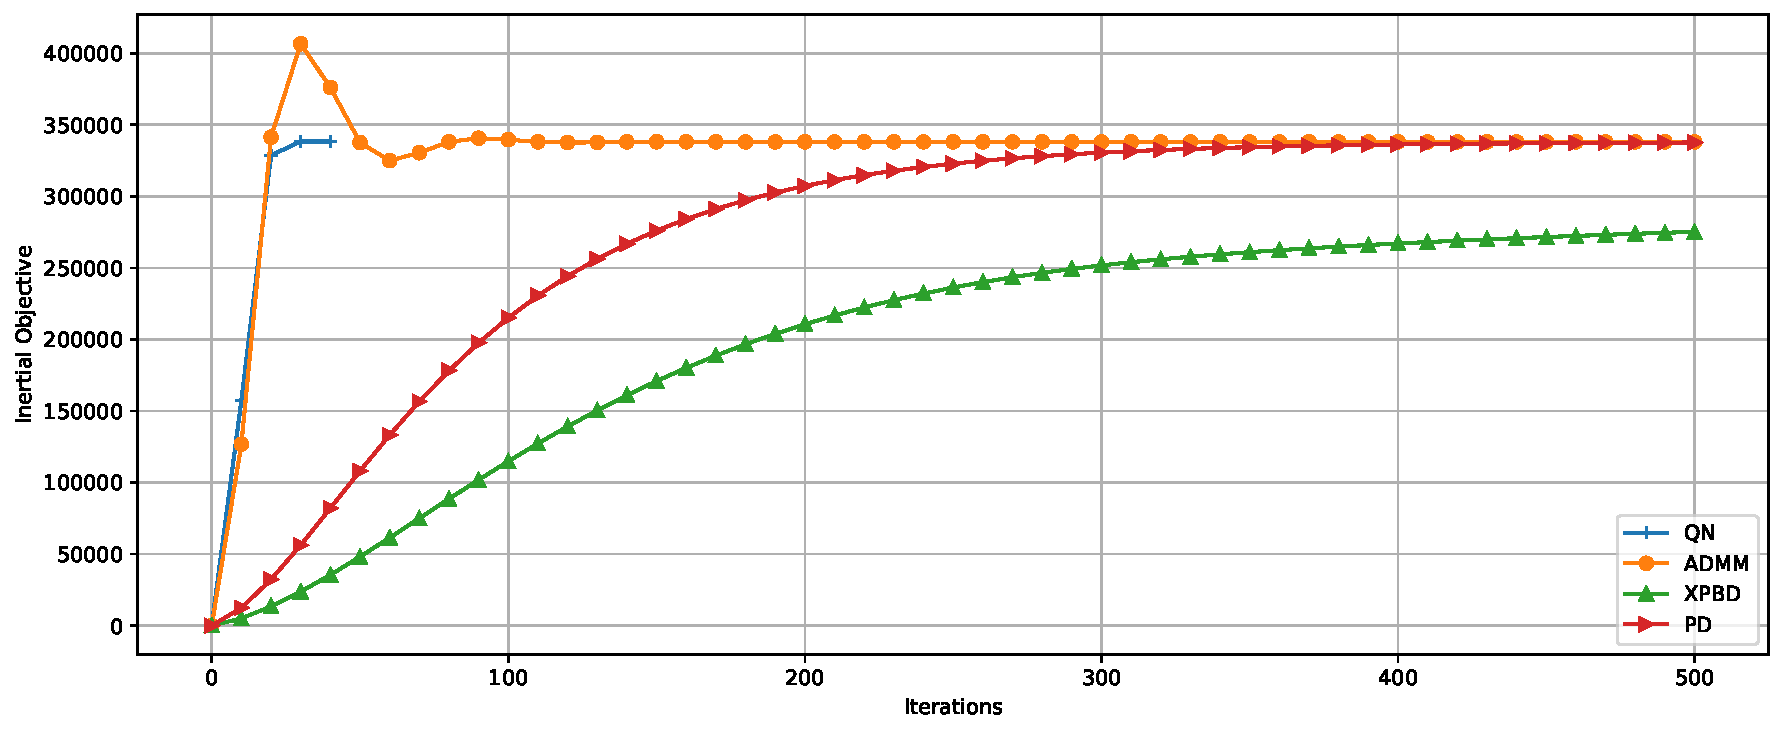
\includegraphics[width=\linewidth]{figures/strain_beam_untwist_inertialObjectives.pdf}
    \end{subfigure}
    \caption{Values of the constraint (top) and inertial (bottom) terms of the objective function of the variational form of implicit Euler integration 
        (see Eq.\ \ref{eq:variational-implicit}) over the iterations of single time step of size \SI{1e-2}{\second} for an untwisting beam with strain 
    constraints with stiffness \num{1e8}.}
    \label{fig:strain-beam-untwist-objectives-split}
\end{figure}

As discussed in Section \ref{ss:variational-implicit-euler}, the weighting between the inertial term and the constraint energy depends on the time step, the particle masses 
and the material stiffnesses. The results suggest that with a time step of \SI{1e-2}{\second} and a constraint stiffness of \num{1e8}, the constraint energy can be 
decreased significantly until the cost of moving particles away from their inertial positions becomes too high. Since the inertial term at the converged XPBD state 
is in fact lower than the inertial term achieved by PD-style solvers, it is evident that the reason for the 
higher objective value of XPBD is that the constraint energy is not reduced sufficiently. It is natural to assume that this 
is in part a consequence of the oscillations resulting from the iterative Gauss-Seidel solver used in XPBD. However, it is worth pointing out again that XPBD does not 
solve the implicit equations of motion exactly due to the simplifying XPBD assumptions. Even if Equation \ref{eq:xpbd-simplified-lse} were to be solved with a global solver,
it is not clear whether the constraint energy would be decreased further than it is using the Gauss-Seidel solver. 

The fact that the constraint energy is higher for the final state of the XPBD solver is also perceptible when comparing its geometry with the final geometries computed 
by PD-style solvers. The geometries achieved after 1000 XPBD and QN iterations are shown in Figure \ref{fig:strain-beam-untwist-geometries} a. 
The corresponding geometries for PD and ADMM are ommitted since they are visually indistinguishable from the geometry computed by the QN solver. The image shows 
that the QN solver untwists the beam further towards its undeformed rest configuration than XPBD. Since the constraint energies obtain a minimum at the reference 
configuration, this is in line with the observation that QN is more successful than XPBD at reducing the constraint term of the objective function. We point out that 
the surface of the XPBD geometry is smooth. In the discussion of Figure \ref{fig:strain-beam-untwist-geometries} b and Figure \ref{fig:twisting-beam-xpbd-failure-geometry},
we suggest that oscillations of the Gauss-Seidel-type solver manifest themselves in noticable geometric artifacts on the beam surface. Thus, it is likely that 
the comparably large constraint term after 1000 XPBD iterations is caused by the simplifying assumptions during the XPBD derivation instead of the local nature of 
the XPBD solver.

Considering that the inertial positions do not appear in the update equations of XPBD (see Sec.\ \ref{ss:xpbd-properties}), it is surprising that the inertial term achieved 
by the converged state of the XPBD solver is smaller than the final inertial term of the other solvers. On the other hand, the only factor driving particles away from 
their inertial positions in the untwisting beam experiment are the elastic energies due to the deformation of the beam. One possible explanation for the low inertial 
term for XPBD might be that the particles do not move far away from their inertial positions simply because the XPBD constraint solver is not as successful at 
minimizing the constraint energies. Lastly, the penalty for moving particles from their inertial positions is quite low for PD-style solvers if a time step as large 
as \SI{1e-2}{\second} is used. However, the inertial term achieved by XPBD remains smaller than its counterparts, even if the timestep is decreased.

\subsection{Conversion of Constraint Energy Into Kinetic Energy}\label{ss:conversion-constraint-kinetic}
In the light of the observation that the inertial term of the objective function of the variational form of implicit Euler integration can be interpreted as the kinetic 
energy of the beam (see Sec.\ \ref{ss:analysis-solvers}), the results in Figure \ref{fig:strain-beam-untwist-objectives-split} suggest that some of the 
constraint energy stored in the deformed beam is converted into kinetic energy during most solver iterations. Additionally, solvers with a 
faster convergence rate appear to be able to convert a larger share of the elastic energy into kinetic energy during a single iteration. 

\subsection{Effects of Early Termination}\label{ss:early-termination}
In the context of real-time applications, the number of solver iterations is often capped to ensure that the computations fit into the time budget allocated 
for the simulation of the next frame. A closer look at Figure \ref{fig:strain-beam-untwist-objectives-split} shows that all of the solvers are still in the process of 
converting the constraint energy stored in the twisted beam into kinetic energy after the first 10 iterations. Accordingly, none of the solvers have reduced the 
objective function to the minimum achieved by the PD-style solvers yet (see Fig. \ref{fig:strain-beam-untwist-objectives}). After 10 iterations, the QN solver has reduced 
the objective function the most, followed by ADMM, PD and XPBD. 

To gain a better understanding of the effects caused by terminating solvers before the objective function is minimized, we take a 
closer look at the geometries that the XPBD, PD and ADMM solvers arrive at after 10 solver iterations in Figure \ref{fig:strain-beam-untwist-geometries} b-d. The 
corresponding QN geometry is given as a reference in each panel. Figure \ref{fig:strain-beam-untwist-geometries} b-d shows that the solvers untwist the beam to 
different extents after the first 10 solver iterations. The QN geometry gets closest to the beam's reference configuration, again followed by ADMM, PD and, lastly, 
XPBD. Note that the degree to which solvers untwist the beam goes hand-in-hand with the extent to which they minimize the objective function and particularly its 
constraint energy. In summary, terminating the solvers after a small number of iterations can cause the motion of simulated bodies to appear slowed down. 
This effect is more noticable for solvers that have inferior convergence properties, such as PD and XPBD. Note that Bouaziz et al.\ \cite{bouaziz2014} report 
the same observation in the discussion of the PD solver and state that this is due to the fact that forces may not be able to fully propagate through the mesh 
if the optimization is not run long enough. 

\begin{figure}
    \centering
    \begin{subfigure}{0.49\textwidth}
        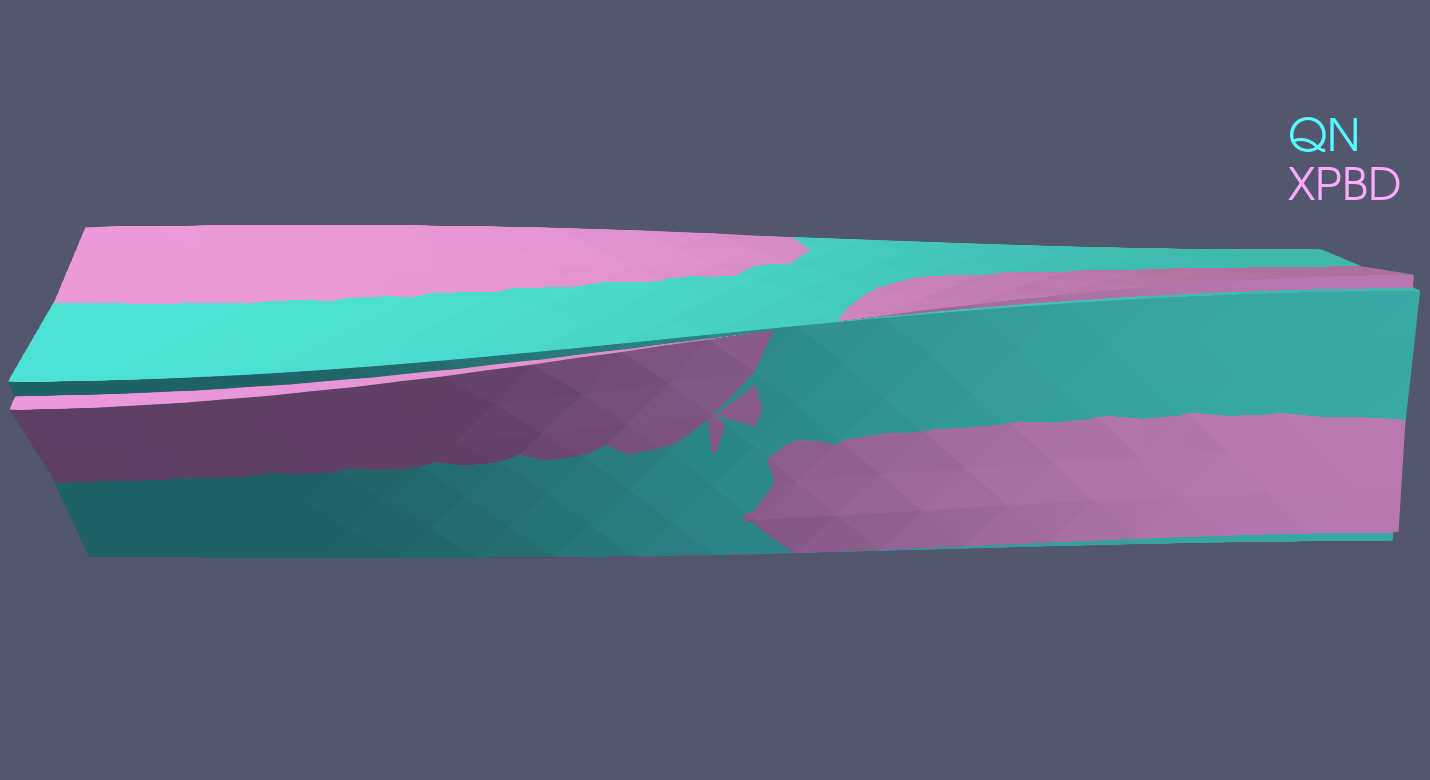
\includegraphics[width=\textwidth, trim={0 5.0cm 0 2.5cm}, clip]{figures/strain_beam_untwist_QN_vs_XPBD.png}
        \subcaption{QN and XPBD after 1000 iterations}
    \end{subfigure}
    \hspace{0.001\textwidth}
    \begin{subfigure}{0.49\textwidth}
        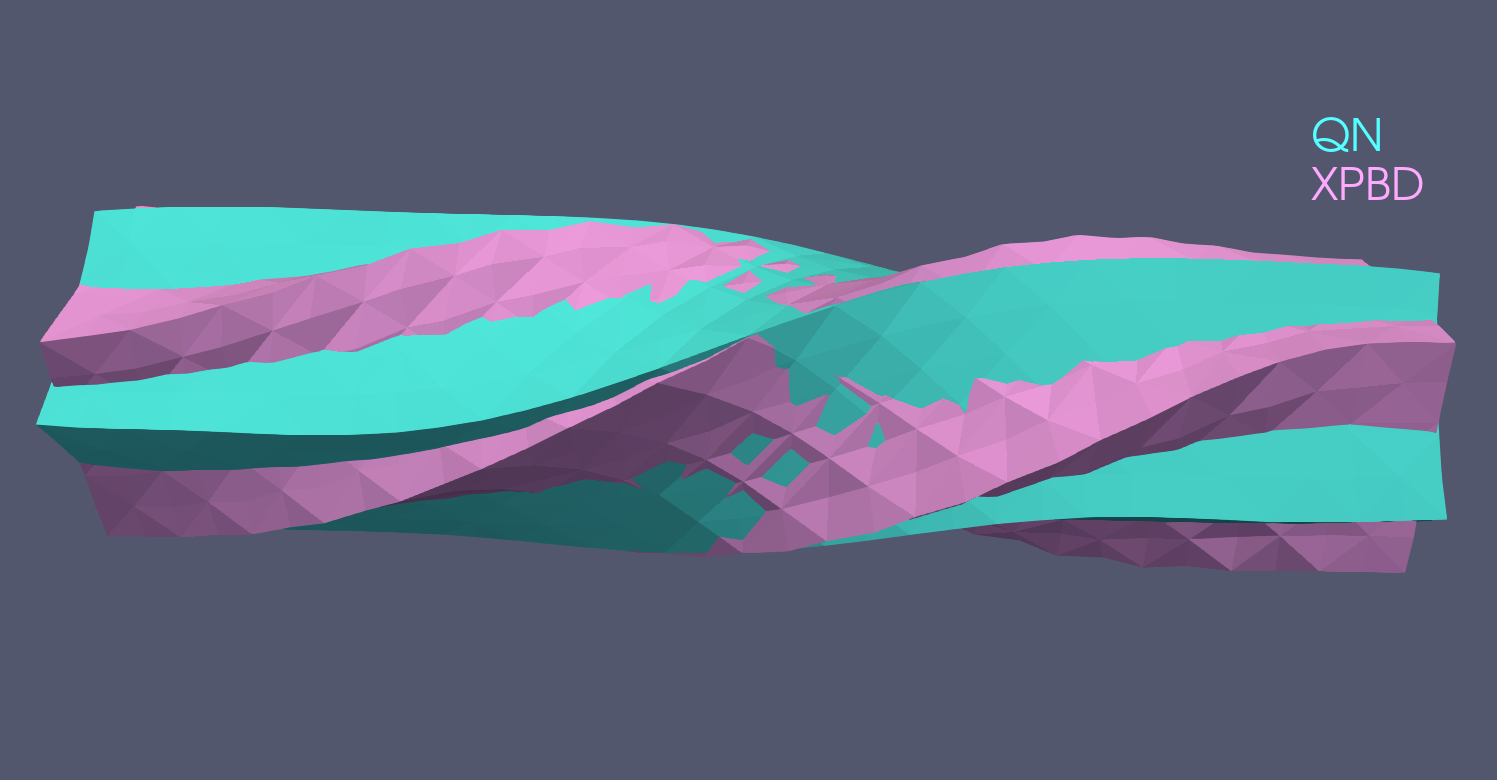
\includegraphics[width=\textwidth, trim={0 4.5cm 0 2.15cm}, clip]{figures/strain_beam_untwist_QN_vs_XPBD_10_iterations.png}
        \subcaption{QN and XPBD after 10 iterations}
    \end{subfigure}
    \par\medskip
    \begin{subfigure}{0.49\textwidth}
        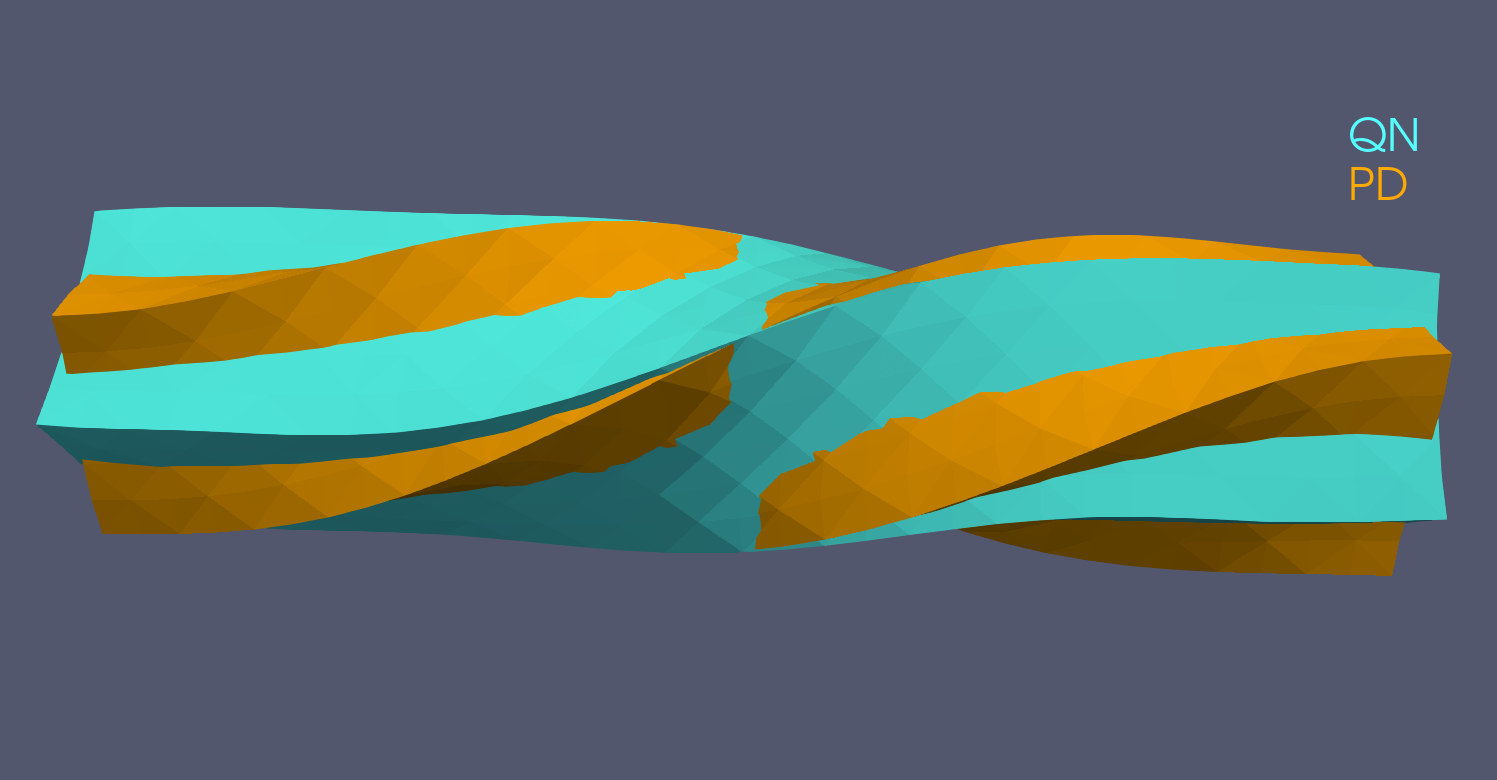
\includegraphics[width=\textwidth, trim={0 4.5cm 0 2.15cm}, clip]{figures/strain_beam_untwist_QN_vs_PD_10_iterations.png}
        \subcaption{QN and PD after 10 iterations}
    \end{subfigure}
    \hspace{0.001\textwidth}
    \begin{subfigure}{0.49\textwidth}
        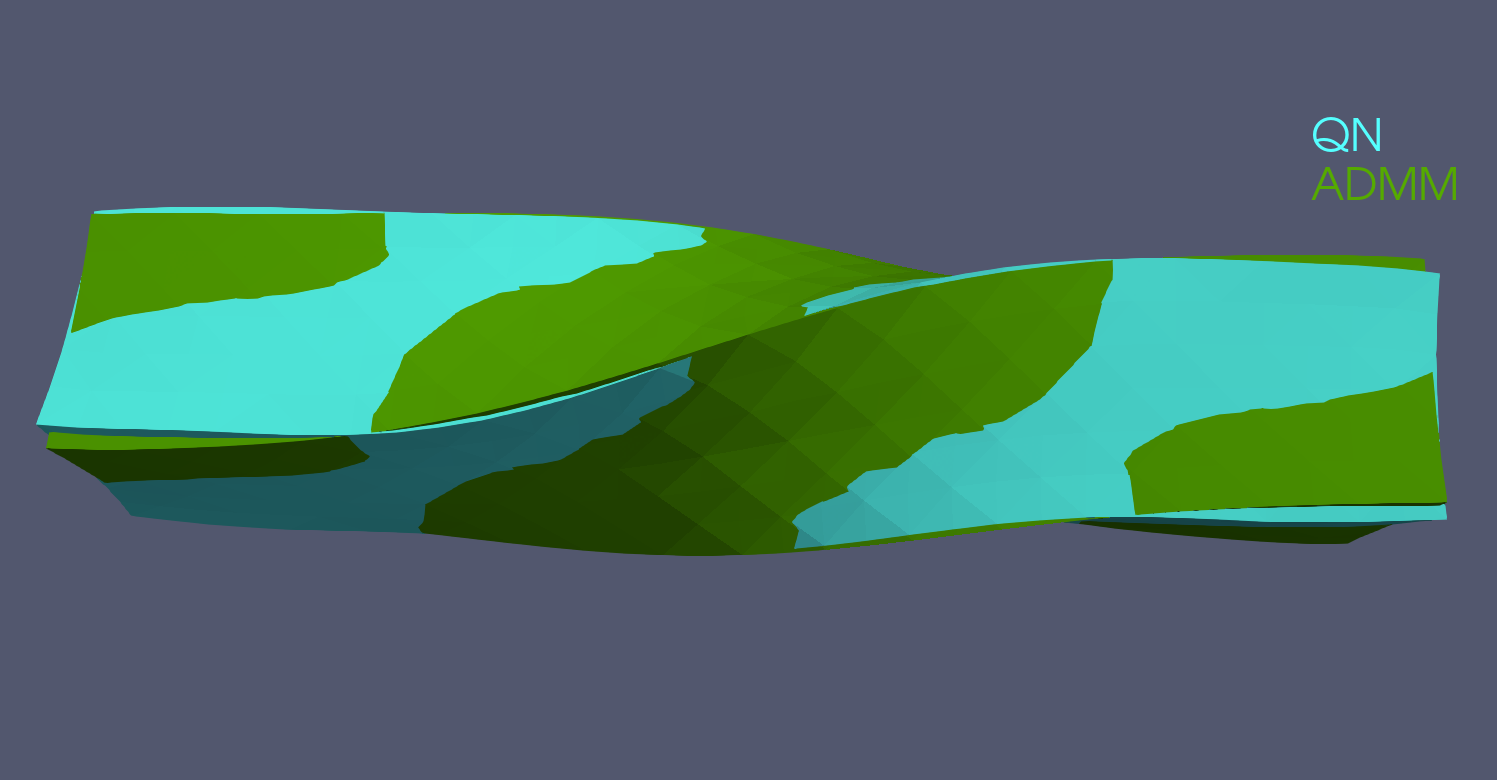
\includegraphics[width=\textwidth, trim={0 4.5cm 0 2.15cm}, clip]{figures/strain_beam_untwist_QN_vs_ADMM_10_iterations.png}
        \subcaption{QN and ADMM after 10 iterations}
    \end{subfigure}
    \caption{Geometries of an untwisting beam with strain constraints (stiffness \num{1e8}) after 10 and 1000 iterations over a single time step of size 
        \SI{1e-2}{\second} using XPBD (pink), PD (orange), ADMM (green) and QN (cyan).}
    \label{fig:strain-beam-untwist-geometries}
\end{figure}

Closer inspection of Figure \ref{fig:strain-beam-untwist-geometries} b shows that the XPBD geometry is noticably rugged compared to the geometries of the PD-type 
solvers, which 
appear mostly smooth at the surface. Thus, in contrast to the PD-style solvers, terminating the simulation early does not only manifest itself in slowing down 
the motion of the simulated body but also in visible geometric artifacts. This matches the observation that the constraint objective value achieved after 10 XPBD iterations 
is larger than the initial constraint objective value in Figure \ref{fig:strain-beam-untwist-objectives-split}. While it is difficult to verify, it is natural to assume that this 
effect is caused by oscillations of the Gauss-Seidel solver at the core of XPBD, since it does not appear for solvers that have a global optimization step. Then, the 
fact that the XPBD geometry does appear smooth after 1000 iterations (see Fig. \ref{fig:strain-beam-untwist-geometries}) would suggest that oscillations are particularly 
severe during earlier iterations where the constraint energies and their gradients are large.

\subsection{Computational Cost}\label{ss:computational-cost-strain}
To take into account the computational cost of the iterations for different solvers, the objective values are plotted again over the accumulated
iteration durations in Figure \ref{fig:strain-beam-untwist-objectives-time}. However, the provided iteration durations should be treated as a rough indication of the 
computational costs of different solvers since no effort has been put into profiling or speeding up the computations by providing a multithreaded 
implementation. The computational costs of XPBD, ADMM and PD seem to very similar on average. 1000 iterations of XPBD, ADMM and PD take roughly 4 seconds each. On the other hand 
QN iterations appear to be almost twice as expensive as the iterations of the other solvers. Still, the conclusions that can be drawn from Figure 
\ref{fig:strain-beam-untwist-objectives-time} are similar to what was discussed for Figure \ref{fig:strain-beam-untwist-objectives}: ADMM and QN converge in a shorter amount 
of time than XPBD and PD, but ADMM and PD appear in a more favorable light compared to QN due to faster iterations.

\begin{figure}[h]
    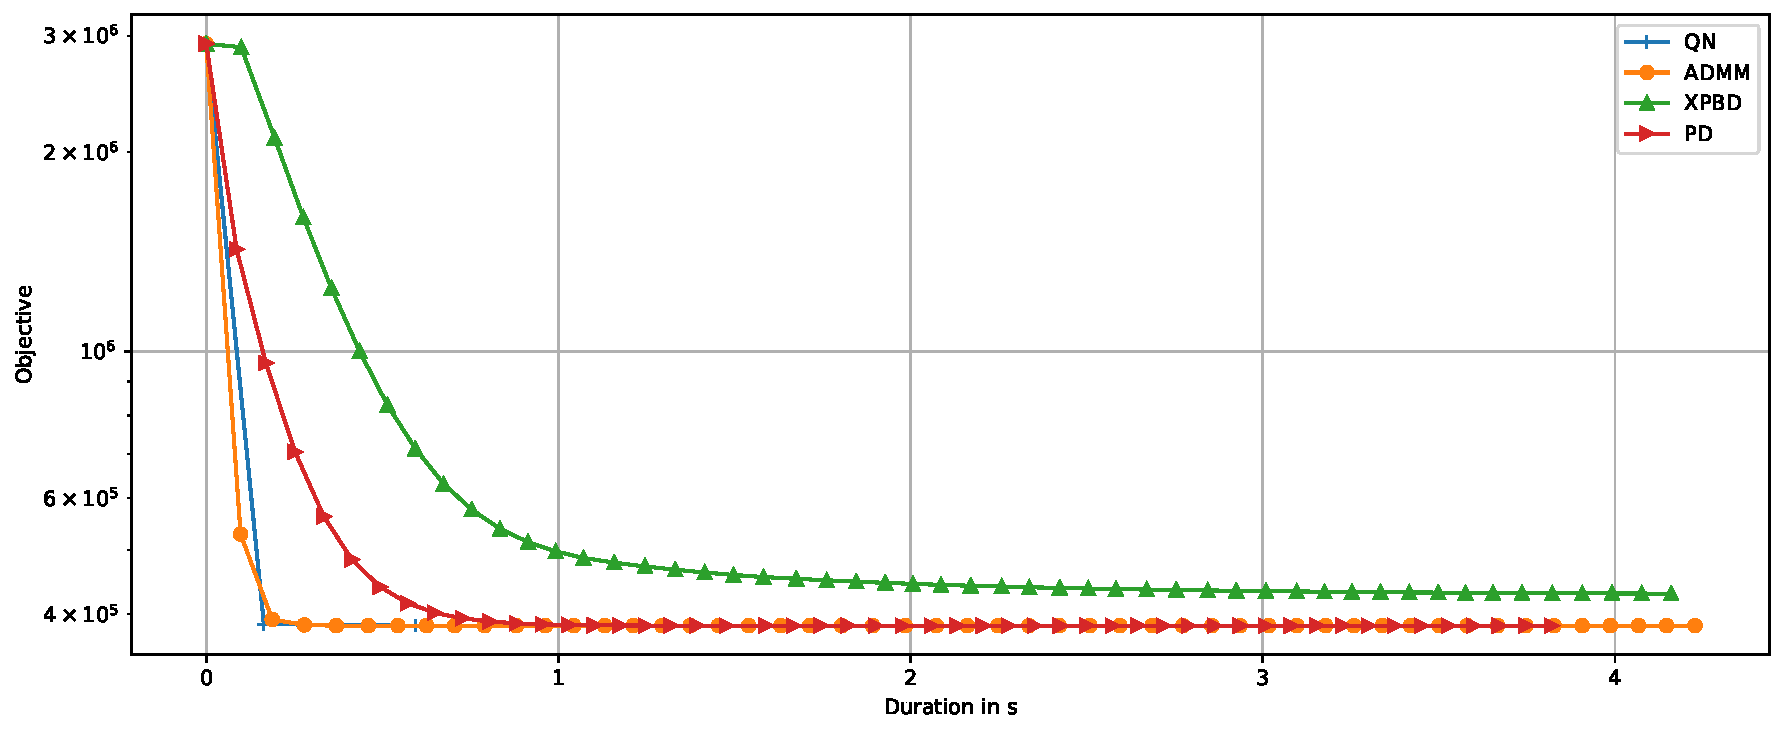
\includegraphics[width=\textwidth]{figures/strain_beam_untwist_objectives_time.pdf}
    \caption{Values of the objective function of the variational form of implicit Euler integration (see Eq.\ \ref{eq:variational-implicit}) over the accumulated durations of 
        the iterations over a single time step of size \SI{1e-2}{\second} for an untwisting beam using strain constraints with stiffness \num{1e8}.}
    \label{fig:strain-beam-untwist-objectives-time}
\end{figure}

\subsection{Convergence Properties With Large Time Steps and Stiffnesses}\label{ss:untwisting-beam-strain-convergence-large-ts}
Figure \ref{fig:strain-beam-untwist-objectives} shows data for time step \SI{1e-2}{\second} and constraint stiffness \num{1e8}. While the results are qualitatively 
the same for a wide range of time steps and stiffness values, noticable differences arise when a combination of large time steps and large stiffness values is used.
Consider the corresponding plot with time step \SI{1e-1}{\second} and constraint stiffness \num{1e9} in Figure \ref{fig:strain-beam-untwist-objectives-large-ts}. Again,
QN makes the fastest progress towards decreasing the objective, followed by ADMM, PD and XPBD. However, from 680 iterations onwards the objective value achieved by the XPBD 
solver is lower than the objective value achieved by the PD solver. In this setting, QN, ADMM and XPBD converge to configurations that achieve roughly the same objective 
function value, while it is PD whose final objective is larger than the other solvers'. After 1000 iterations, PD has a relative error (see Eq.\ \ref{eq:rel-error}) 
of approx.\ 0.02 \%. While this appears negligible, it is worth noting that the minimal objective value that PD arrives at is still approx.\ 2.3 
times larger than the minimal value achieved by the other solvers.


\begin{figure}[h]
    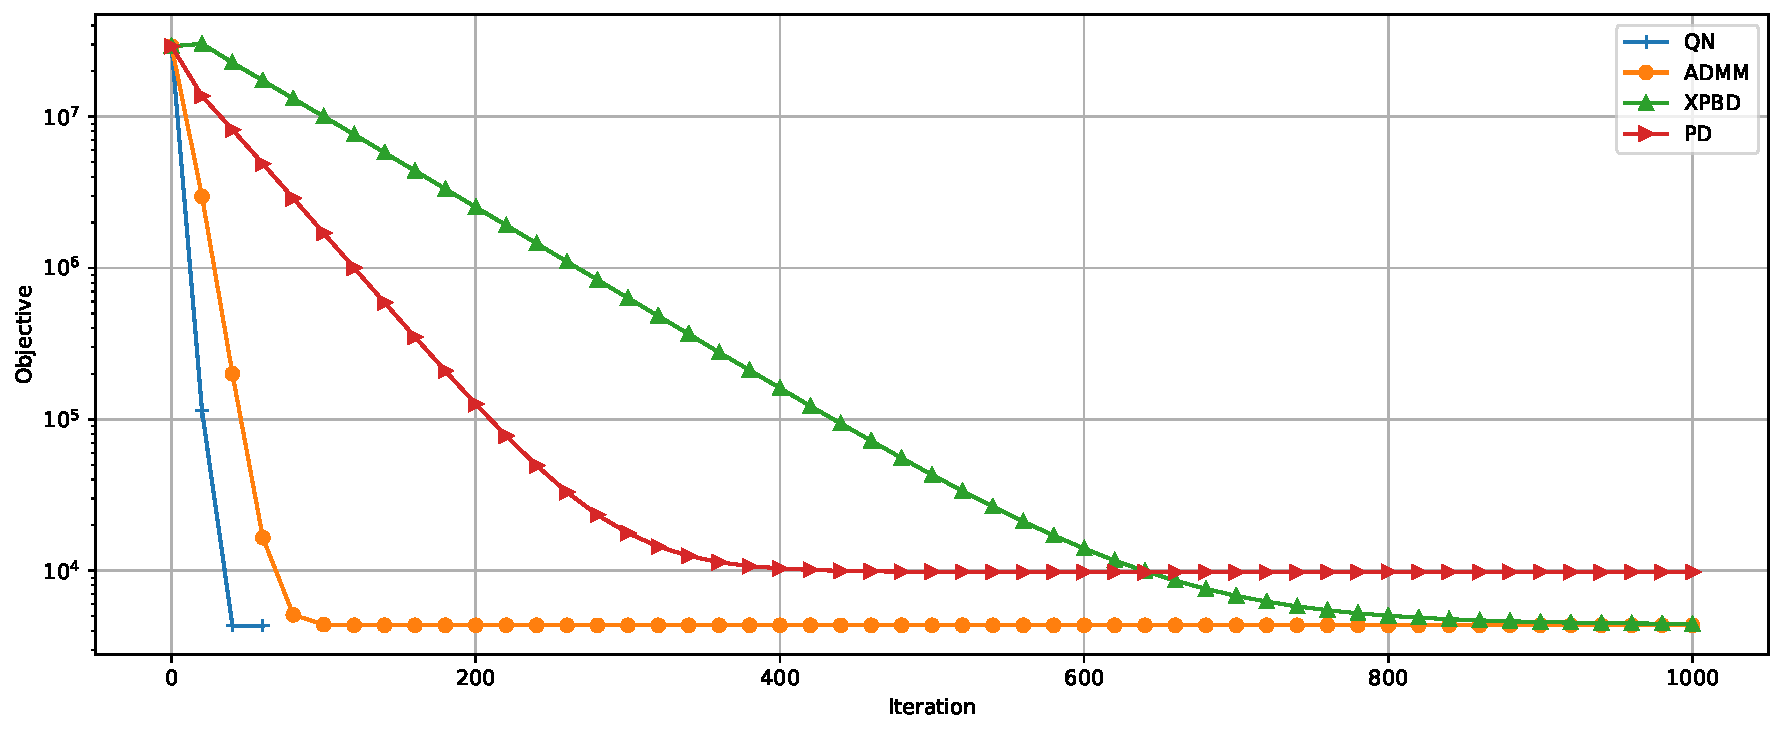
\includegraphics[width=\textwidth]{figures/strain_beam_untwist_objectives_large_ts.pdf}
    \caption{Values of the objective function of the variational form of implicit Euler integration (see Eq.\ \ref{eq:variational-implicit}) over the iterations of a single time 
        step of size \SI{1e-1}{\second} for an untwisting beam using strain constraints with stiffness \num{1e9}.}
    \label{fig:strain-beam-untwist-objectives-large-ts}
\end{figure}

As discussed in Section \ref{ss:pd-properties}, each PD iteration is guaranteed to weakly reduce the objective function. However, this only ensures that the objective function 
at the configuration PD converges to is never higher than the initial objective value. There is no guarantee that 
PD converges to the true implicit positions. Thus, the observation that PD can fail at reducing the objective function all the way is not surprising. To gain a better 
understanding of why the convergence properties of the PD solver worsen when combining larger time steps and stiffness values, we again create separate plots for the 
inertial and constraint terms. This is analogous to the experiments conducted in Figure \ref{fig:strain-beam-untwist-objectives-split} to investigate 
the unfavorable convergence properties of XPBD observed in Figure \ref{fig:strain-beam-untwist-objectives}. 

\begin{figure}[t]
    \centering
    \begin{subfigure}{\textwidth}
        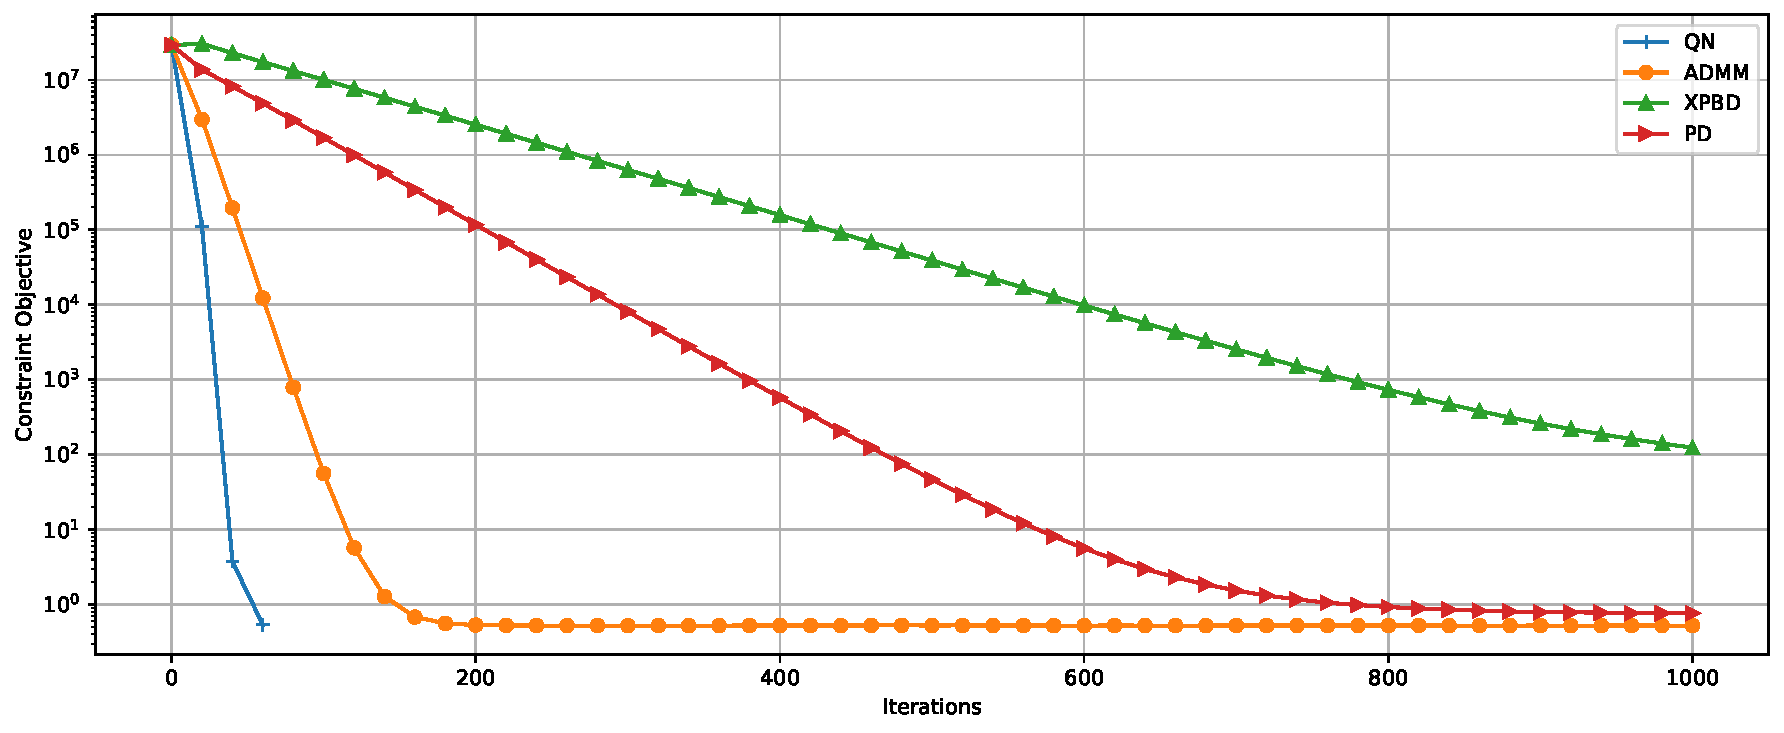
\includegraphics[width=\linewidth]{figures/strain_beam_untwist_constraintObjectives_large_ts.pdf}
    \end{subfigure}
    \begin{subfigure}{\textwidth}
        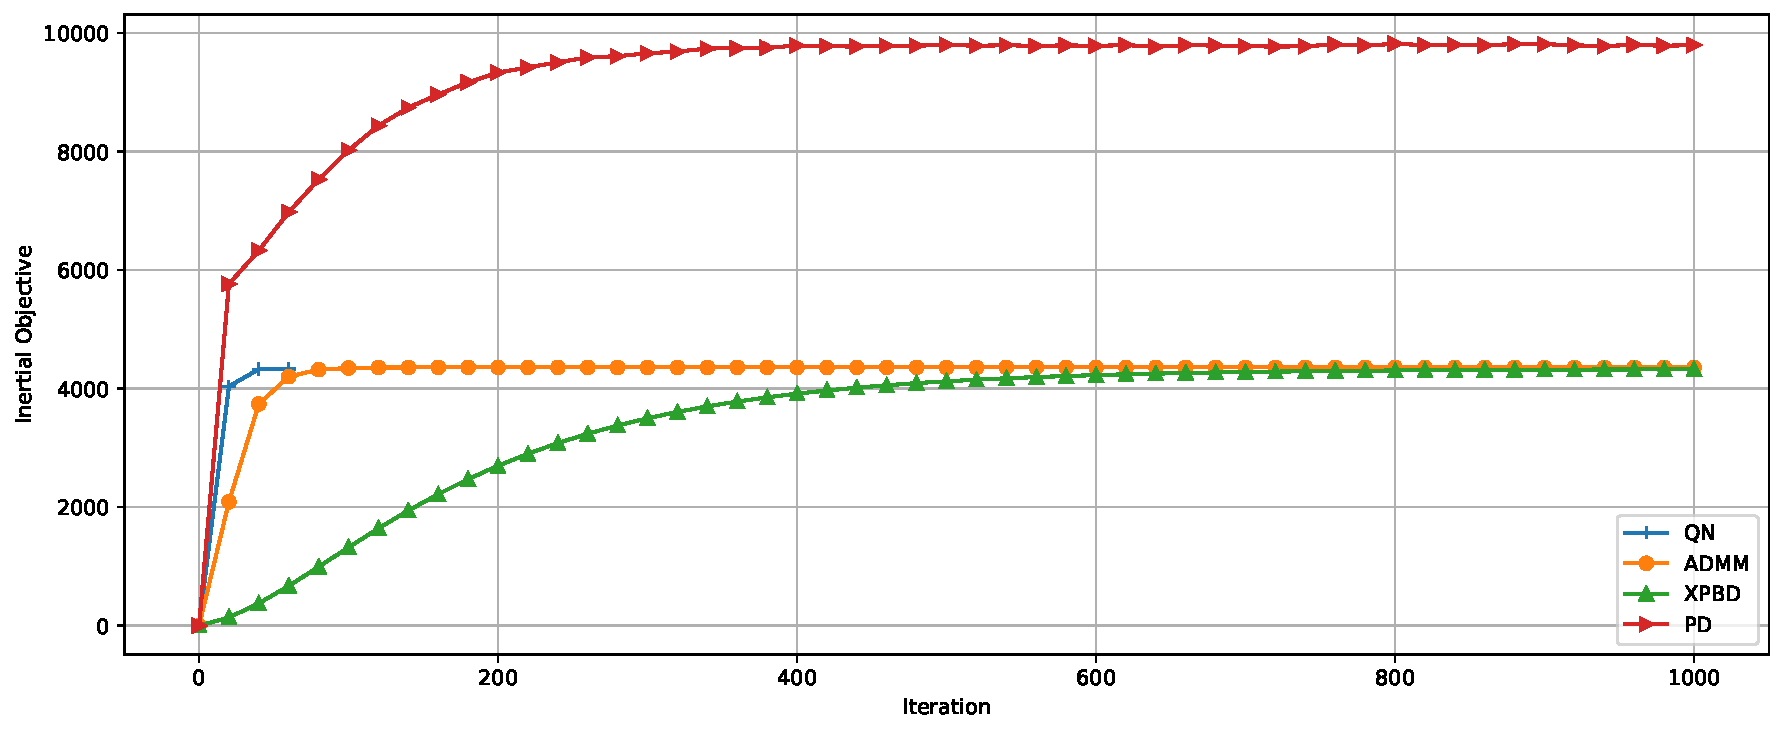
\includegraphics[width=\linewidth]{figures/strain_beam_untwist_inertialObjectives_large_ts.pdf}
    \end{subfigure}
    \caption{Values of the constraint (top) and inertial (bottom) terms of the objective function of the variational form of implicit Euler integration 
        (see Eq.\ \ref{eq:variational-implicit}) over the iterations of a single time step of size \SI{1e-1}{\second} for an untwisting beam using strain constraints with 
    stiffness \num{1e9}.}
    \label{fig:strain-beam-untwist-objectives-split-large-ts}
\end{figure}

Again, Figure \ref{fig:strain-beam-untwist-objectives-split-large-ts} shows that the solvers mostly decrease the constraint term and increase the inertial term during each 
iteration. QN, ADMM and PD are more successful at reducing the constraint energy than XPBD, even 
though PD converges to a constraint energy that is slightly larger than the one achieved by QN and ADMM this time. Each of the PD-style solvers manages to bring the 
constraint energy down to close to zero. This is significantly lower than the minimum achieved for a time step of \SI{1e-2}{\second} and stiffness \num{1e8} (see 
Fig. \ref{fig:strain-beam-untwist-objectives-split}). However, it is evident that XPBD has not fully converged yet as it still continues to decrease the constraint energy 
values. All in all, the results for the constraint energy are qualitatively the same as the ones observied for 
time step \SI{1e-2}{\second} and stiffness \num{1e8}. On the other hand, the plots for the inertial term differ quite significantly. With larger time step and stiffness,
QN, ADMM and XPBD converge to roughly the same inertial term, whereas the PD solver converges to a value that is more than twice as large. Already after 20 iterations, 
the inertial term achieved by PD is larger than the value that the other solvers converge to. Still, PD continues to increase the inertial term during the first 400 
iterations. Finally, each of the solvers converge to an inertial term that is significantly lower than the corresponding inertial term obtained with time step 
\SI{1e-2}{\second} and stiffness \num{1e8}.

Since the weight of the inertial term decreases with increasing time step size and the weight of the constraint term increases with increasing stiffness values, moving 
particles away from their inertial positions to reduce the constraint energy is encouraged in Figure \ref{fig:strain-beam-untwist-objectives-split-large-ts} compared to
Figure \ref{fig:strain-beam-untwist-objectives-split}. This is reflected in the fact that the solvers reduce the constraint energy to a lower value, even though a larger 
stiffness value is used. The results suggest that the PD solver is too aggressive with moving particles away from their inertial positions if the associated penalty 
is largely outweighed by the incentives for minimizing the constraint energies. This issue 
appears to be particularly serious during the first solver iterations, where the derivatives of the quadratic inertial penalty are small. 
Without further experiments, it is difficult to understand why this effect occurs when using the PD solver while the other solvers are unaffected.

\subsection{Conservation of Global Linear and Angular Momentum With Large Time Steps and Stiffnesses}\label{ss:momenta-large-ts}
To gain further insights into the cause of the large inertial term at the converged configuration from PD, we repeat parts of the 
experiments in Figure \ref{fig:strain-beam-untwist-geometries} and take a closer look at the geometries that the solvers arrive at after 1000 
iterations. Figure \ref{fig:strain-beam-untwist-geometries-large-ts} a shows a comparison between the XPBD and QN geometries. Similar to the 
results in Figure \ref{fig:strain-beam-untwist-geometries} a, the XPBD solver does not untwist the beam as far as the QN solver. This is in 
line with the observation that the constraint term for XPBD is larger than the constraint term of PD-style solvers after 1000 iterations (see 
Figure \ref{fig:strain-beam-untwist-objectives-split-large-ts}). More interestingly, the comparison of the QN, ADMM and PD geometries in 
Figure \ref{fig:strain-beam-untwist-geometries-large-ts} b shows that all PD-style solvers succeed at untwisting the beam to its reference 
configuration. However, while the orientations of the beams appear the same between solvers, the positions of their centers of gravity 
are shifted with respect to each other. This shift is very apparent for PD, whereas the QN and ADMM geometries are almost overlapping.

The results in Figure \ref{fig:strain-beam-untwist-geometries-large-ts} suggest that the large inertial term observed for the PD solver in 
Figure \ref{fig:strain-beam-untwist-objectives-split-large-ts} is caused by undesired rigid-body motion introduced during the solver iterations. 
The shifted center of gravity of the beam is unexpected in light of the fact that the beam has zero global linear and angular momentum in 
its initial twisted configuration and no external forces are applied. At the true implicit positions that the PD solver attempts to converge to, global 
linear and angular momentum are preserved \cite{bouaziz2014}. However, the shifted center of gravity indicates that the global linear 
momentum of the beam is non-zero after 1000 PD iterations.

\begin{figure}
    \centering
    \begin{subfigure}{0.49\textwidth}
        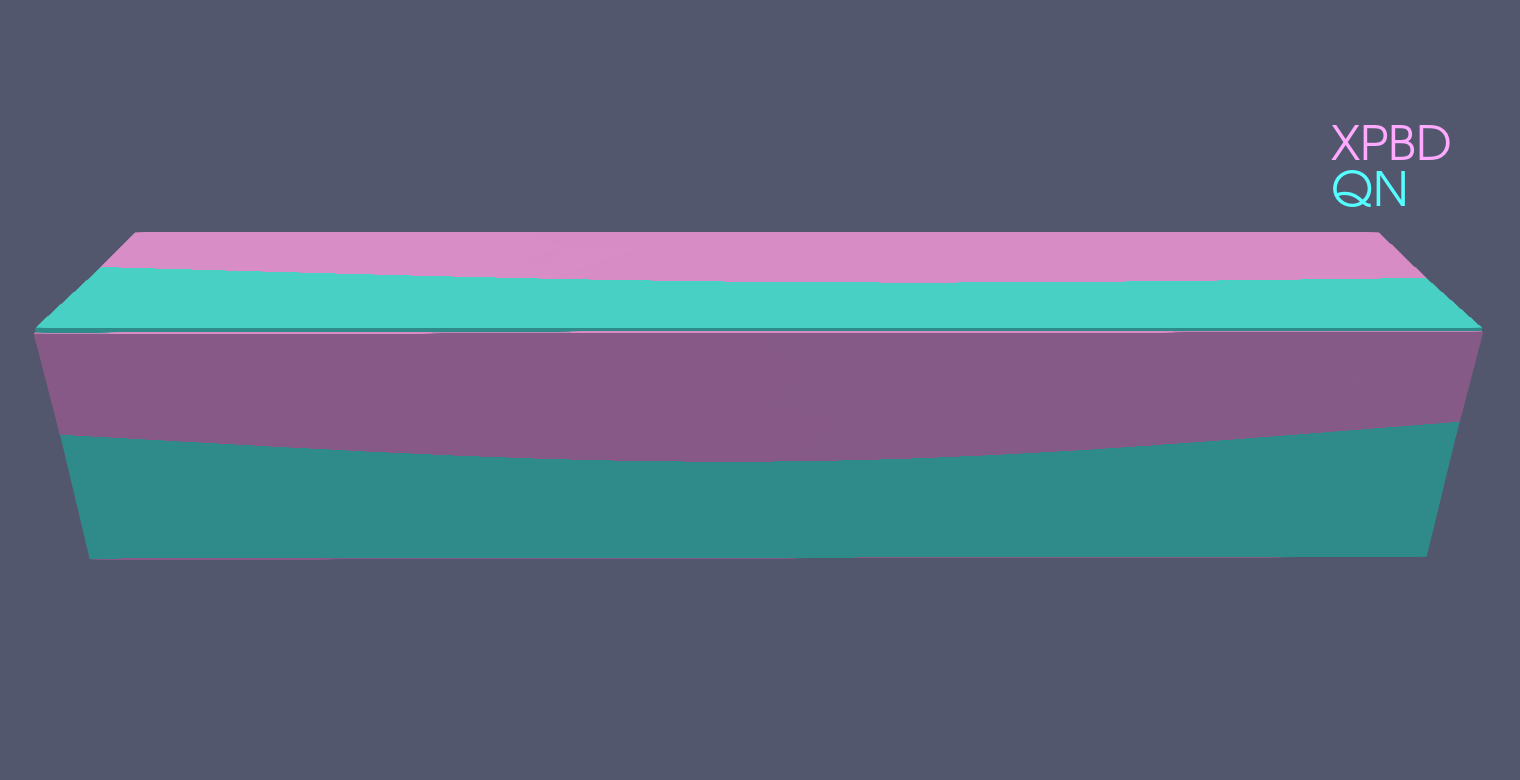
\includegraphics[width=\textwidth, trim={0 5.0cm 0 2.5cm}, clip]{figures/strain_beam_untwist_QN_vs_XPBD_large_ts.png}
        \subcaption{QN and XPBD after 1000 iterations}
    \end{subfigure}
    \hspace{0.001\textwidth}
    \begin{subfigure}{0.49\textwidth}
        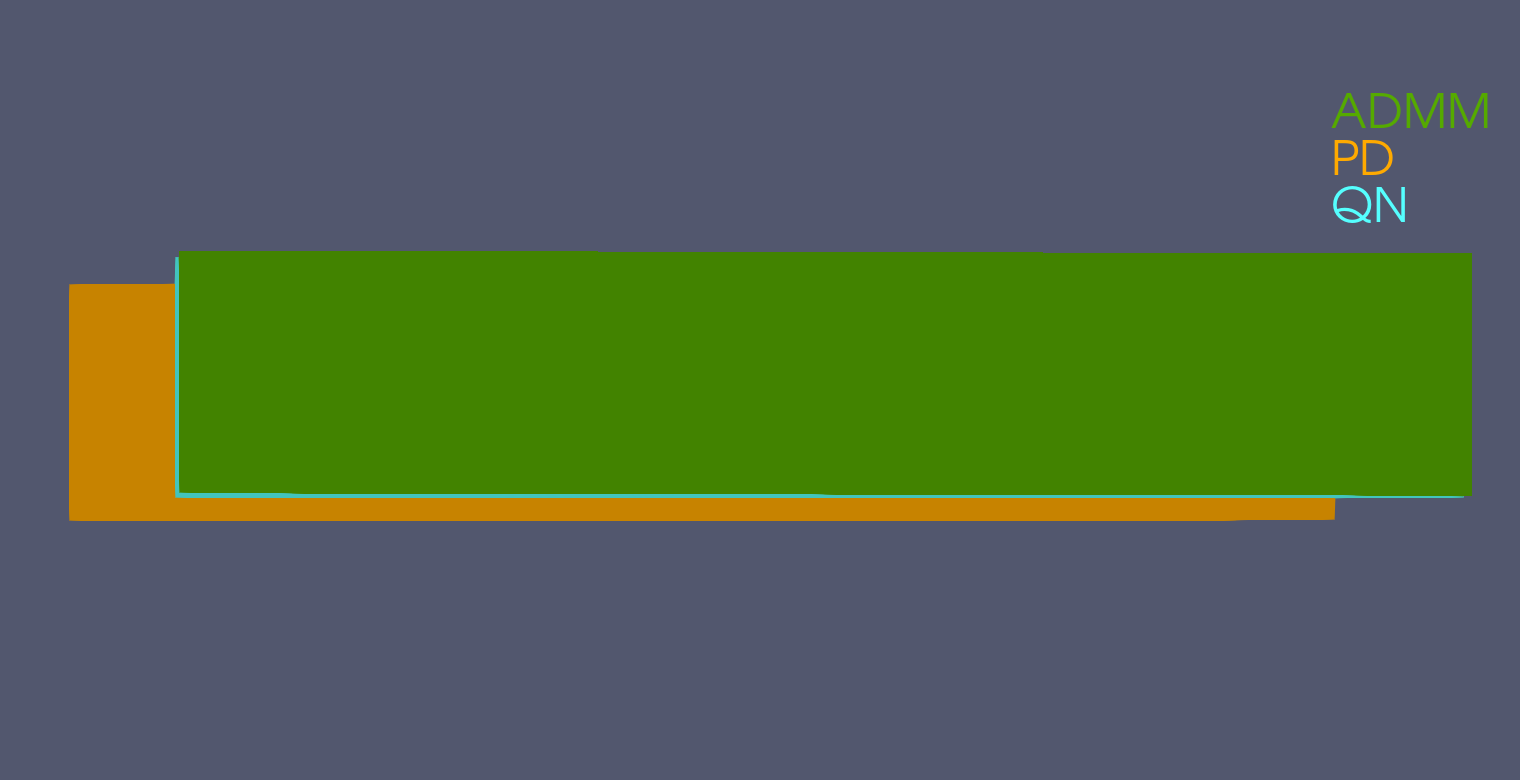
\includegraphics[width=\textwidth, trim={0 4.5cm 0 2.15cm}, clip]{figures/strain_beam_untwist_QN_vs_ADMM_vs_PD_large_ts.png}
        \subcaption{QN, PD and ADMM after 1000 iterations}
    \end{subfigure}
    \caption{Geometries of an untwisting beam with strain constraints (stiffness \num{1e9}) after 1000 iterations over a single time step of size 
    \SI{1e-1}{\second} using XPBD (pink), PD (orange), ADMM (green) and QN (cyan).}
    \label{fig:strain-beam-untwist-geometries-large-ts}
\end{figure}

To dig deeper, we plot the norms of the global linear and angular momentum of the beam over the solver iterations in 
Figure \ref{fig:strain-beam-untwist-momenta-large-ts}. First, the plots confirm that the initial linear and angular momenta are zero at the initial 
configuration. However, the QN solver is the only solver that succeeds at preserving both types of momentum. XPBD preserves linear momentum, 
but increases the angular momentum. PD and ADMM fail to preserve either type of momentum. The bulk of the 
increase in linear momentum observed for PD and ADMM happens during the first 20 iterations. The final linear momentum observed for the PD solver is 
significantly larger than the one observed for the other solvers. During the rest of the iterations, the linear momentum remains almost constant for all solvers. 
It is worth pointing out that the plot for the linear momentum is representative for the corresponding plots for almost all combinations of time step size and 
constraint stiffness. On the other hand, the plots for the angular momentum are more varied. The main commonality is that the angular momentum norms are much 
smaller than the linear momentum norms observed for PD and ADMM solvers. For these reasons, we focus our attention on linear momentum. 

First, the data provides insight into why the spike of the inertial term of the objective function after 20 PD iterations in 
Figure \ref{fig:strain-beam-untwist-objectives-split-large-ts} does not go along with a large decrease in the constraint term: The spike is caused by 
rigid-body motion, to which elastic energy potentials are invariant. Secondly, we discussed in Section \ref{ss:pd-quasi-newton} that PD can be considered 
a quasi-Newton method with constant Hessian approximation. The QN solver enhances the PD solver by integrating local curvature information into the Hessian 
approximation via an LBFGS update and adding a line search algorithm. Since the QN solver does not introduce any global linear momentum, it follows that
the reason for the PD solver's inability to preserve the linear momentum is the lack of one or both of these features of the QN solver. To find out which of 
these factors is more important, it might be interesting to remove the line search or the LBFGS-update from the QN solver and take another look at the momenta. 
Lastly, recall that ADMM and PD are almost identical for strain constraints if the ADMM weights $w_i$ are set to $\sqrt{k}$. For the experiments in 
Figure \ref{fig:strain-beam-untwist-momenta-large-ts}, $w_i \approx \frac{1}{2}\sqrt{k}$ is used. Thus, the smaller linear momentum observed for ADMM invites 
the hypothesis that lower ADMM weights can be beneficial for the preservation of linear momentum. However, more effort is required to verify this claim and 
to establish the causal justification. 

\begin{figure}[h]
    \centering
    \begin{subfigure}{\textwidth}
        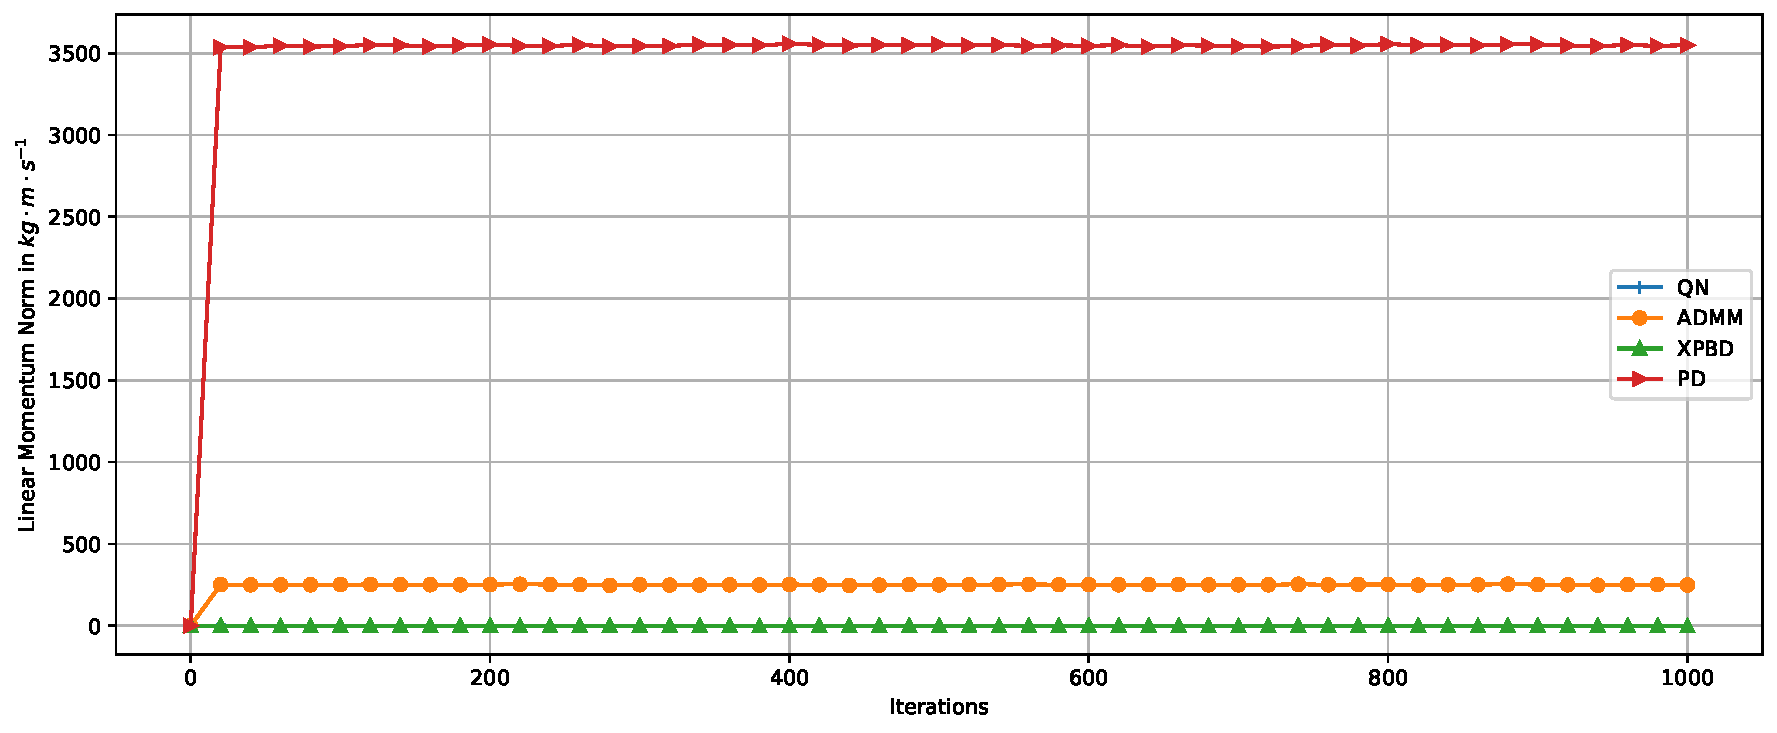
\includegraphics[width=\linewidth]{figures/strain_beam_untwist_momenta_large_ts.pdf}
    \end{subfigure}
    \begin{subfigure}{\textwidth}
        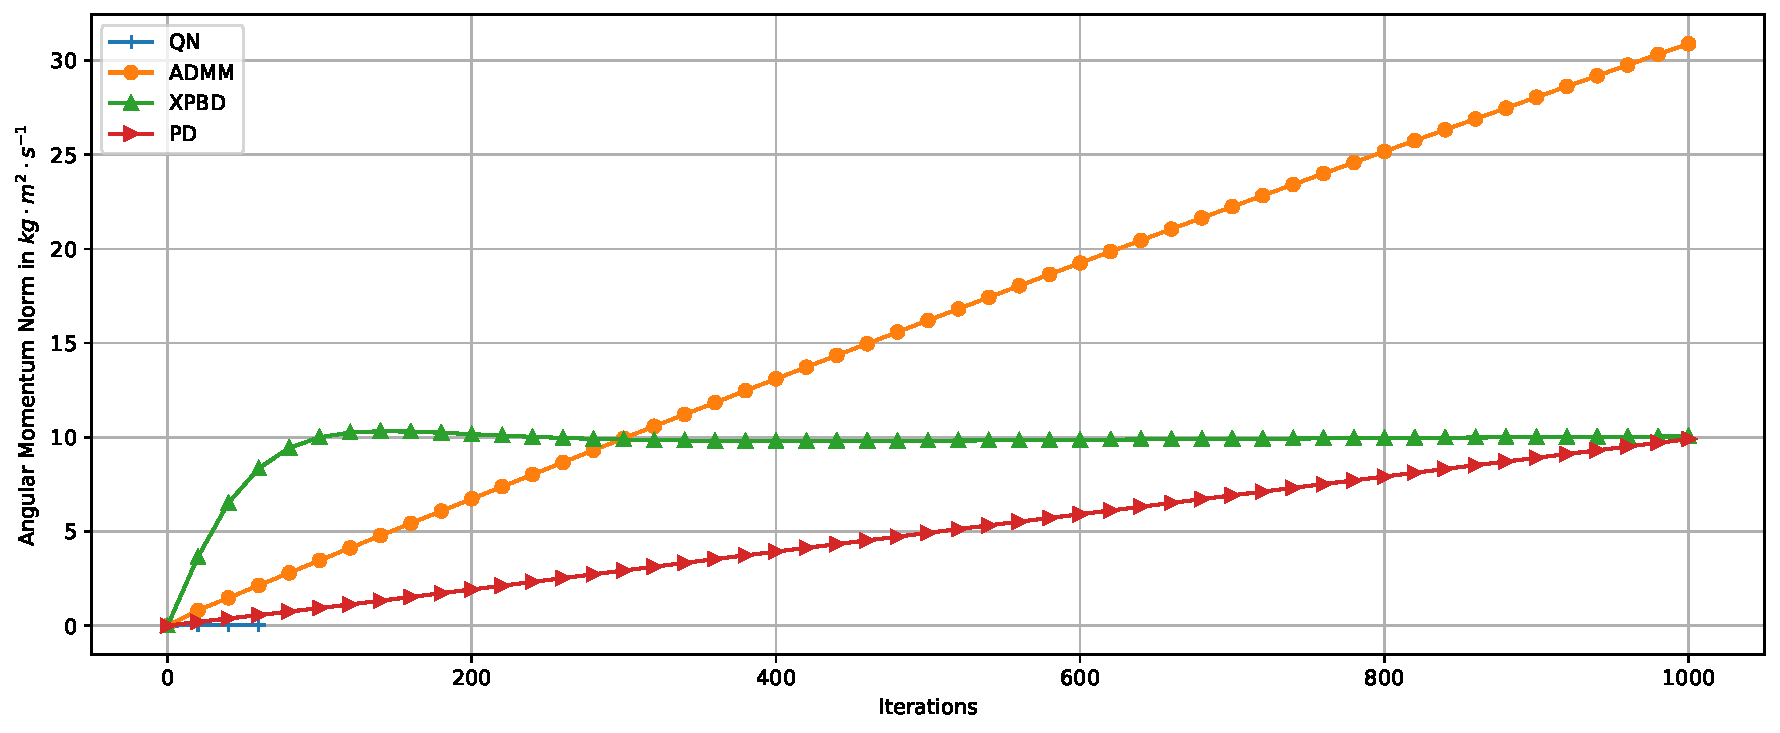
\includegraphics[width=\linewidth]{figures/strain_beam_untwist_angular_momenta_large_ts.pdf}
    \end{subfigure}
    \caption{Norms of the global linear (top) and global angular (bottom) momenta in $\text{kg}\cdot\text{m}^2\cdot\text{s}^{-1}$ over the iterations 
    of a single time step of size \SI{1e-1}{\second} for an untwisting beam with strain constraints with stiffness \num{1e9}. The required velocities 
    $\vecm{v}_k$ at iteration $k$ are computed via Verlet integration (see Sec.\ \ref{ss:analysis-solvers}).
}
    \label{fig:strain-beam-untwist-momenta-large-ts}
\end{figure}

\section{Twisting Beam Simulations - Strain Material}\label{ss:twisting-beam-strain}
In the twisting beam experiment, the twisting motion of the beam is achieved by position constraints whose reference positions are rotated in-plane at the 
ends of the beam. These position constraints and the tetrahedral constraints for the strain material model are incompatible in the sense that there are no 
positions $\vecm{q}$ for which all constraint energies are minimized at the same time. Thus, the twisting beam experiments put the the solvers' abilities 
to make compromises between competing constraints to the test. The ADMM weights for the twisting beam experiments are reused from the parameter screens 
for the untwisting beam experiments. We start by giving an overview of the convergence properties of different solvers in the twisting beam experiments in 
Section \ref{ss:twisting-beam-strain-convergence}. Relevant details for the XPBD and ADMM solvers are discussed in Sections \ref{ss:twisting-beam-xpbd} and 
\ref{ss:twisting-beam-admm}.

\subsection{Overview Over Convergence Properties}\label{ss:twisting-beam-strain-convergence}
To gain insights into the convergence properties of the solvers in the twisting beam examples, we again start by plotting the objective values over 
the solver iterations. The resulting graphs for a time step size of \SI{1e-1}{\second} and a stiffness value of \num{1e9} are shown in 
Figure \ref{fig:strain-beam-twist-typical-objectives}. While the results obtained for the QN and PD solvers are qualitatively the same for all time step 
sizes and stiffness values, the behavior of XPBD and ADMM can vary quite dramatically across different parameter settings. The plots in 
Figure \ref{fig:strain-beam-twist-typical-objectives} show that both QN and PD converge to a configuration with a lower objective value than the initial 
objective value within the first 20 iterations. Note that it takes a larger number of iterations to achieve convergence in the corresponding untwisting beam experiments 
(see Fig. \ref{fig:strain-beam-untwist-objectives-large-ts}). This is particularly noticable for the PD solver. Figure \ref{fig:strain-beam-twist-typical-objectives} 
shows that ADMM exhibits the same behavior as QN and PD for time step \SI{1e-1}{\second} and stiffness \num{1e9}. While this can be observed for a variety of 
different parameter settings, there are also many cases where ADMM either does not converge at all or converges to a solution whose objective value is 
significantly lower than the objective value achieved by the other PD-style solvers. Lastly, XPBD converges to a configuration with an objective value that is 
significantly larger than the initial objective value in Figure \ref{fig:strain-beam-twist-typical-objectives}. Again, this observation is repeated for a variety of 
different parameters. However, there are also combinations of time step sizes and stiffness values for which XPBD is successful at reducing the objective to 
below its initial value. Even in such settings, the minimal objective value achieved by XPBD is almost always higher than the one achieved by QN and PD.

\begin{figure}[h]
    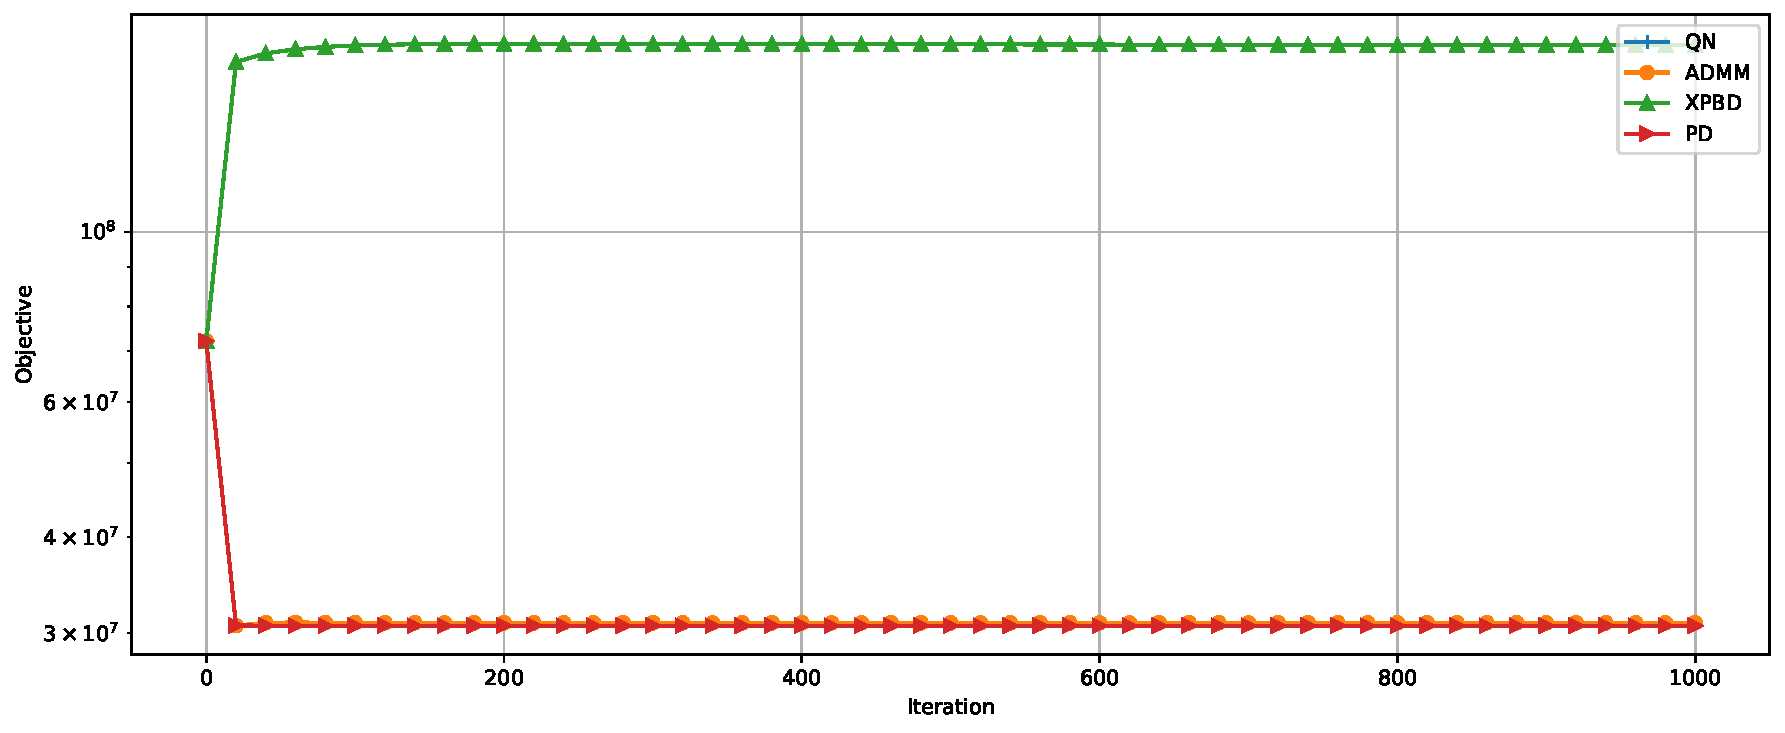
\includegraphics[width=\textwidth]{figures/strain_beam_twist_typical_objectives.pdf}
    \caption{Values of the objective function of the variational form of implicit Euler integration (see Eq.\ \ref{eq:variational-implicit}) over the iterations of 
        a single time step of size \SI{1e-1}{\second} for a twisting beam using strain constraints with stiffness \num{1e9}.}
    \label{fig:strain-beam-twist-typical-objectives}
\end{figure}

During the discussion of the untwisting beam experiments using large time steps and stiffness values (see Fig.\ \ref{fig:strain-beam-untwist-objectives-large-ts}),
we pointed out that the PD solver can fail to decrease the objective value to the value achieved by the QN solver. This is caused by the introduction of 
undesired rigid-body motion during early PD iterations when the penalty for moving particles away from their inertial positions is largely outweighed by the incentives 
for minimizing constraint energies. Since the position constraints at the ends of the beam in the twisting beam experiments further disincentivize moving the beam's 
center of gravity, it is not surprising that this failure mode of the PD solver is not encountered. The fact that convergence is achieved after fewer iterations 
during the twisting beam experiments than during the unwisting beam experiments is expected considering that the initial particle positions are much closer to the true 
implicit positions that the solvers aim to converge. To see this, observe that the QN solver untwists the beam from its initial deformed configuration all the way to its 
undeformed reference configuration over a single time step in Figure \ref{fig:strain-beam-untwist-geometries-large-ts} b. In contrast, the beam is only twisted by a 
couple of degrees during the twisting beam experiments. As mentioned earlier, the results for XPBD and ADMM are more complex and merit a more detailed discussion below.

\subsection{Convergence Properties of XPBD}\label{ss:twisting-beam-xpbd}
During the untwisting beam experiments using the strain material model discussed earlier, each solver reduces 
the objective value compared to the initial objective value during the first 1000 iterations, irrespective of the chosen time step size 
and stiffness value. As indicated by the data in  Figure \ref{fig:strain-beam-twist-typical-objectives}, this is not always the case for the twisting beam experiments. 
For various combinations of time step sizes and stiffness values, the positions computed by XPBD after 1000 iterations yield a higher objective function 
value than the initial objective value. We say that XPBD fails for such parameters. For each time step, the stiffness values for which XPBD fails are listed in 
Figure \ref{fig:strain-beam-twist-xpbd-failures}. Note that the results are identical when restricting to the constraint term of the objective function. 
In other words, the settings in which XPBD fails to decrease the objective are exactly those for which the solver iterations cause the constraint 
term to increase. Figure \ref{fig:strain-beam-twist-xpbd-failures} shows that XPBD fails in settings where large stiffness 
values are used. In particular, XPBD always fails once the stiffness is larger than some time step dependent threshold. This threshold 
increases with increasing time step size.

\begin{table}[h]
\centering
    \begin{tabular}{ |r||c|c|c|c| } 
     \hline
     time step in s & \num{1e-1} & \num{1e-2} & \num{1e-3} & \num{1e-4}\\ 
     \hline
     stiffness & $\geq$ \num{1e7} & $\geq$ \num{1e8} & $\geq$ \num{1e10} & $\geq$ \num{1e12}\\
     \hline
    \end{tabular}
    \caption{Combinations of time step sizes and stiffness values for which XPBD fails. For a stiffness value $k$, we write $\geq k$ to indicate that 
        XPBD fails for all tested stiffnesses $k^\prime$ such that $k^\prime > k$. Identical results are obtained when restricting to the constraint 
        term of the objective function.
    }
\label{fig:strain-beam-twist-xpbd-failures}
\end{table}

As discussed before, the large constraint terms that are observed when XPBD fails are most likely caused by a combination of the simplifying 
assumptions during the XPBD derivation and oscillations of the Gauss-Seidel-type solver at its core. We assess that the latter contributes 
more to XPBD failures in the twisting beam experiments for a variety of reasons. First, it is easy to see how mixing incompatible 
position and strain constraints could lead to more severe oscillations. Since there are no particle positions $\vecm{q}$ for which both the position constraints and the 
strain constraints are satisfied at the same time, individual constraint projections will continue to move particles back and forth over and over again. 
On the other hand, all strain constraints are satisfied in the reference configuration of the beam in the untwisting beam scenario. It is natural to 
assume that the former scenario is more challenging for Gauss-Seidel-type solvers. Secondly, the severity of the oscillations is expected to increase with both 
time step size and stiffness values since both factors enable larger position updates during individual constraint projections. This is in line with the 
data presented in Figure \ref{fig:strain-beam-twist-xpbd-failures}.

To get a feeling for the visual effects resulting from the large (constraint) objective value achieved when XPBD fails, we take a closer look at the 
geometry of a twisting strain beam after 1000 XPBD iterations over a time step of \SI{1e2}{\second} with constraint stiffness \num{1e12} in 
Figure \ref{fig:twisting-beam-xpbd-failure-geometry}. The left panel shows that the surface of the XPBD geometry is noticably rugged. Recall that 
the same observation is made after 10 XPBD iterations in the untwisting beam setting (see Fig. \ref{fig:strain-beam-untwist-geometries}). The 
effect is particularly noticable at the ends of the beam, where individual tetrahedra protrude from the volume of the body. To highlight this, 
we zoom in on the geometry at one end of the beam in the right panel of Figure \ref{fig:twisting-beam-xpbd-failure-geometry}. The geometry that the QN solver 
converges to is given as a reference. While the QN geometry is flat at the end of the beam, the XPBD geometry is irregular. Additionally, it 
appears that the end of the beam is twisted further in the counterclockwise direction when using the XPBD solver.

\begin{figure}[h]
    \resizebox{\textwidth}{!}{
    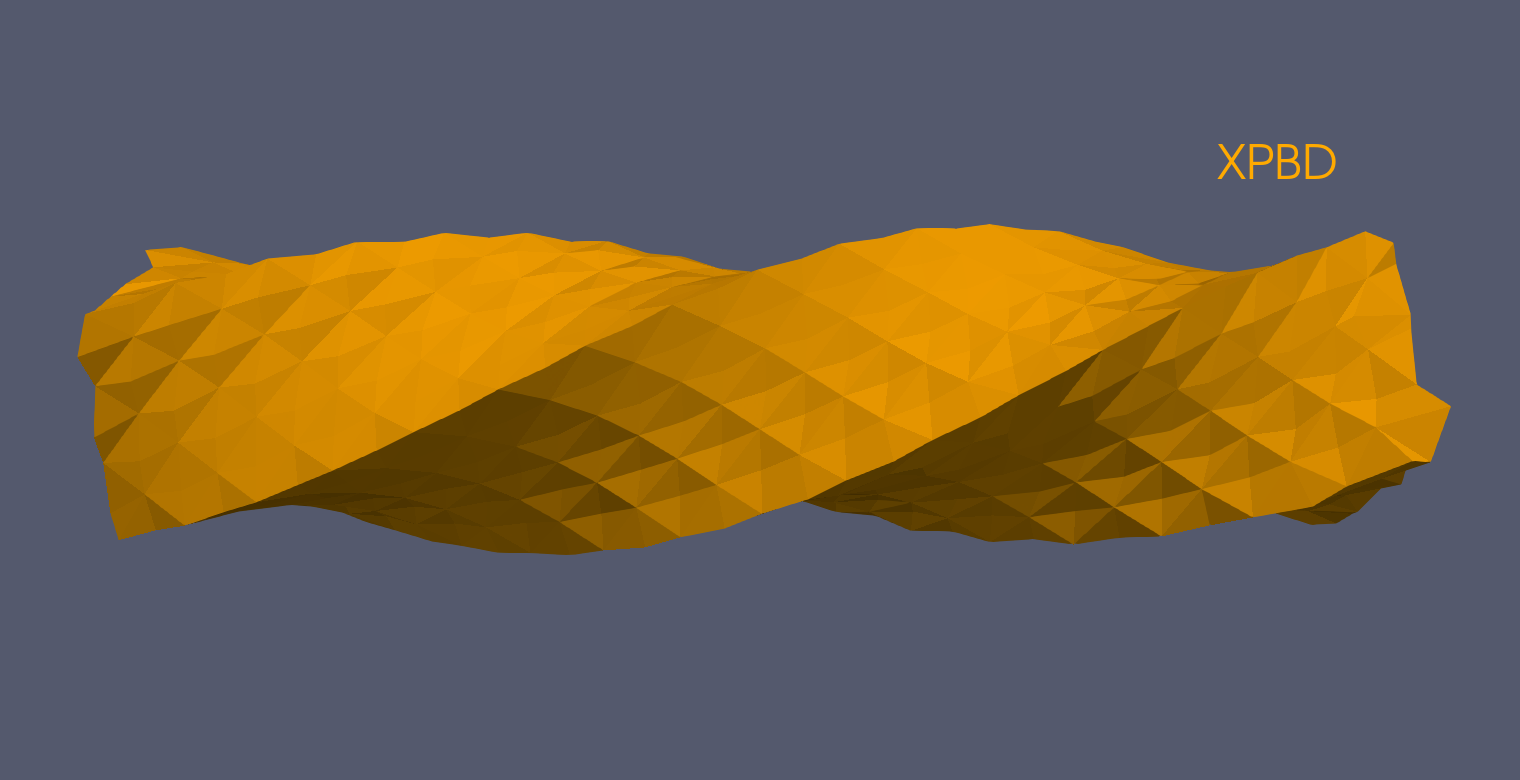
\includegraphics[height=10cm, trim={0 5.0cm 0 2.5cm}, clip]{figures/twisted_beam_rugged_xpbd.png}
    \quad
    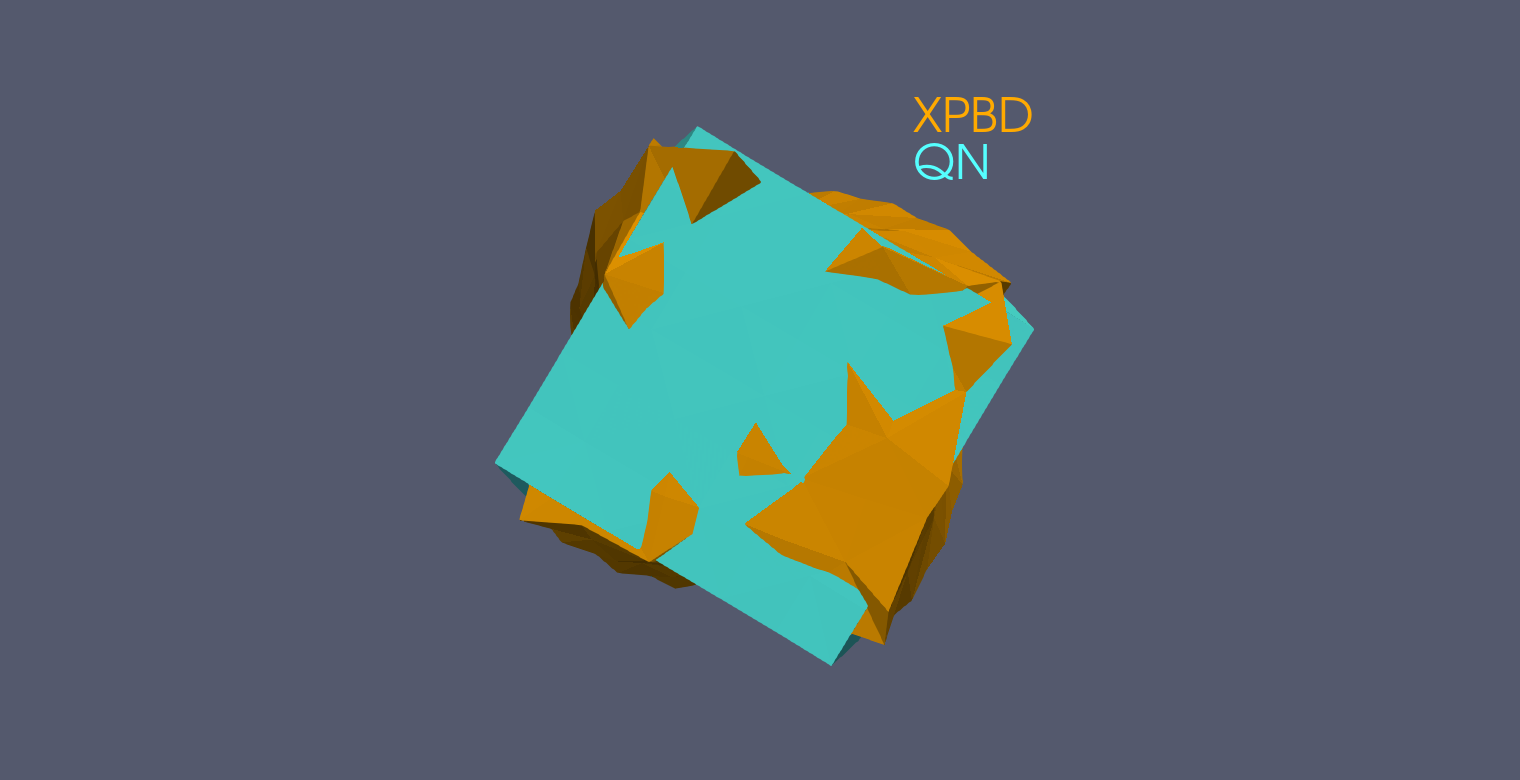
\includegraphics[height=10cm, trim={16.5cm 2.0cm 15.5cm 2.0cm}, clip]{figures/twisted_beam_sideview.png}
    }
    \caption{Geometries of a twisting beam with strain constraints (stiffness \num{1e12}) after 1000 XPBD iterations over a time step of size \SI{1e-2}{\second} 
    from different angles. In the right panel, the converged QN geometry is shown as a reference.}
    \label{fig:twisting-beam-xpbd-failure-geometry}
\end{figure}

Again, the observed rugged surface fits with our hypothesis that the failures of the XPBD solver in the twisting beam scenario are due to 
oscillations of the Gauss-Seidel-type solver at the core of XPBD. The protrusions at the end of the beam are most likely caused by oscillations 
between the incompatible position constraints and local strain constraints. Together, our results from Figure \ref{fig:strain-beam-untwist-geometries} and 
Figure \ref{fig:twisting-beam-xpbd-failure-geometry} suggest that oscillations can cause noticable geometric artifacts if an insufficiently low number of 
XPBD iterations is used or if subsets of constraints are fundamentally incompatible. The observation that the beam is twisted further from its 
initial configuration for XPBD than for QN is expected considering that the XPBD solver has no explicit penalty for moving particles away from their inertial 
positions (see Sec.\ \ref{ss:xpbd-properties}). Thus, XPBD has more freedom to update particle positions in such a way that the position constraints 
that cause the beam to twist are satisfied. On the other hand, moving particles away from their inertial positions is associated with a penalty that is 
quadratic in the inverse of the time step size when using the QN solver. As a result, the final QN positions at the end of the beam are further 
away from the reference positions of the position constraints. While the behavior of the QN solver is physically accurate, it 
also highlights one of its weaknesses: Due to the penalty incurred for moving particles away from their inertial positions and the fact that 
position constraints can only be modelled via stiff springs, exerting exact control over a set of particle positions is challenging. Note that even the 
large stiffness value of \num{1e12} used for the position constraints in Figure \ref{fig:twisting-beam-xpbd-failure-geometry} is insufficient for moving particles 
to their reference positions when using the QN solver.

\begin{table}[h]
\centering
    \begin{tabular}{ |r||c|c|c|c| } 
     \hline
     time step in s & \num{1e-1} & \num{1e-2} & \num{1e-3} & \num{1e-4}\\ 
     \hline
     stiffness & -- & $\geq$ \num{1e5} & $\geq$ \num{1e5} & $\geq$ \num{1e7}\\
     \hline
    \end{tabular}
\caption{Combinations of time step sizes and stiffness values for which the inertial term of XPBD is larger than the inertial term of the QN solver after 
1000 iterations.}
\label{fig:strain-beam-twist-xpbd-large-inertial-terms}
\end{table}

The fact that the XPBD solver is more liberal with moving particles at the ends of the beam towards the reference positions of the position constraints 
should be reflected in a larger inertial term compared to the QN solver. In Figure \ref{fig:strain-beam-twist-xpbd-large-inertial-terms}, we list combinations 
of time step sizes and stiffness values for which the inertial term after 1000 XPBD iterations is larger than the inertial term achieved at the converged 
QN configuration. The results show that XPBD's inertial term is always smaller when a time step of \SI{1e-1}{\second} is used, but almost always larger for 
time step sizes larger than or equal to \SI{1e-2}{\second}. The only exception occurs for small stiffness values when a time step of \SI{1e-4}{\second} is 
used.

The results are in line with the observations from the previous experiments. In particular, Figure \ref{fig:strain-beam-twist-xpbd-large-inertial-terms} shows 
that the inertial term achieved by XPBD is larger than the inertial term achieved by QN for the parameters used in 
Figure \ref{fig:twisting-beam-xpbd-failure-geometry} (time step \SI{1e-2}{\second}, stiffness \num{1e12}). The observation that the inertial term achieved by 
the QN solver is larger for the large time step \SI{1e-1}{\second} matches that the inertial penalty taken into account by the QN solver 
is quadratic in the inverse of the time step size. As this penalty is not reflected in the XPBD update equations, it is expected 
that XPBD's inertial term becomes larger than QN's inertial term when the time step is reduced. 

In our discussion of Figure \ref{fig:strain-beam-untwist-objectives-split}, we mentioned that the inertial term achieved by 
XPBD is almost always lower than the inertial term achieved by PD-style solvers in the untwisting beam experiment. We suggested that this is due to the 
fact that the tetrahedral strain constraints simply do not provide enough incentive to move particles away from their inertial positions and that XPBD is 
less successful at minimizing the constraint energies of the tetrahedral elements than PD-style solvers. On the other hand, the position constraints at 
the end of the twisting beam are associated with quadratic spring energies that are simple to optimize and do encourage moving particles 
away from their inertial positions. In this setting, the lack of an explicit penalty term in the XPBD update equations becomes evident.

\begin{figure}[h]
    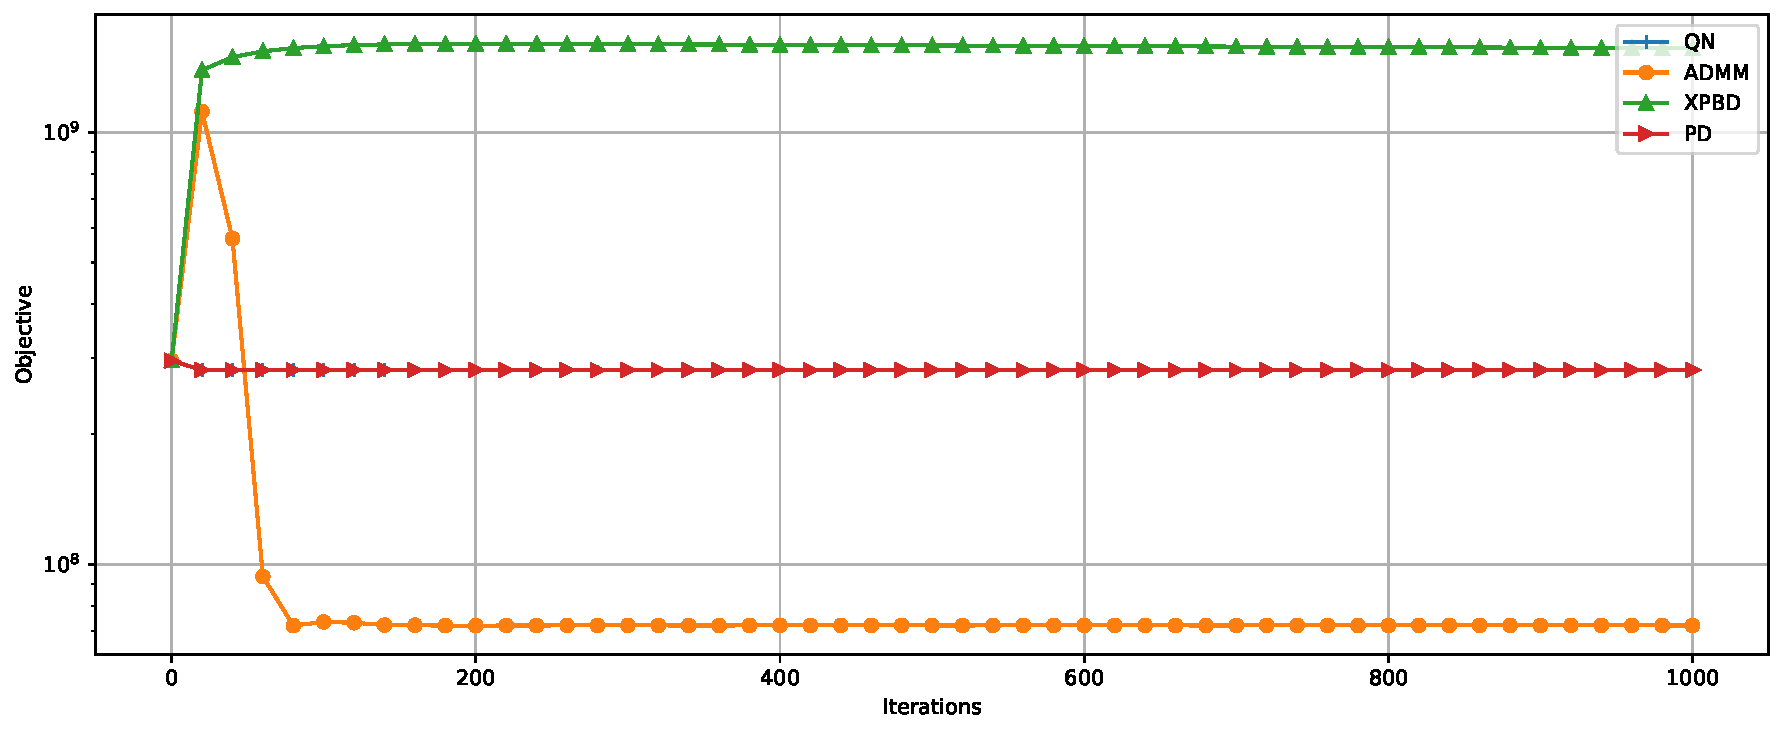
\includegraphics[width=\textwidth]{figures/strain_beam_twist_objectives.pdf}
    \caption{Values of the objective function of the variational form of implicit Euler integration (see Eq.\ \ref{eq:variational-implicit}) over the iterations of 
        a single time step of size \SI{1e-2}{\second} for a twisting beam using strain constraints with stiffness \num{1e10}.}
    \label{fig:strain-beam-twist-objectives}
\end{figure}

\subsection{Convergence Properties of ADMM}\label{ss:twisting-beam-admm}
For some parameters, we observe that ADMM converges to a configuration for which the objective value is significantly lower than the objective values 
achieved by all other solvers during the twisting beam experiments. As an example, we plot the objective values over the iterations for a time step of 
\SI{1e-2}{\second} and stiffness \num{1e10} in Figure \ref{fig:strain-beam-twist-objectives}. After increasing the objective value during the first 40 
iterations, the ADMM solver arrives at a lower objective value than the initial objective value after 60 iterations. Finally, ADMM 
converges to a configuration where the objective value is almost an order of magnitude lower than the minimal objective value achieved by PD and QN after 
80 iterations.

\begin{figure}[t]
    \centering
    \begin{subfigure}{\textwidth}
        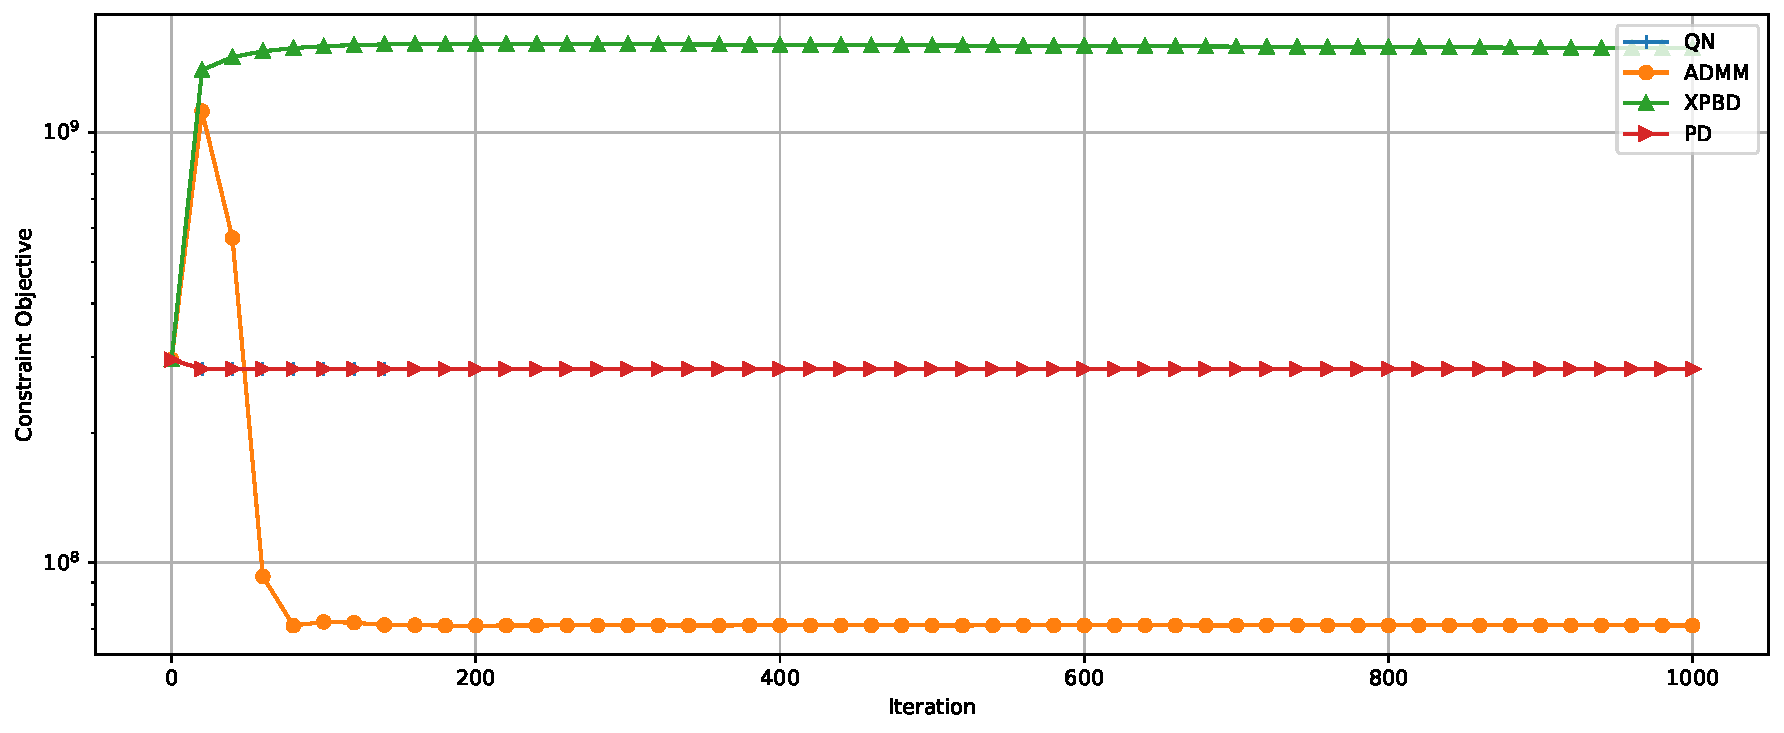
\includegraphics[width=\linewidth]{figures/strain_beam_twist_constraintObjective.pdf}
    \end{subfigure}
    \begin{subfigure}{\textwidth}
        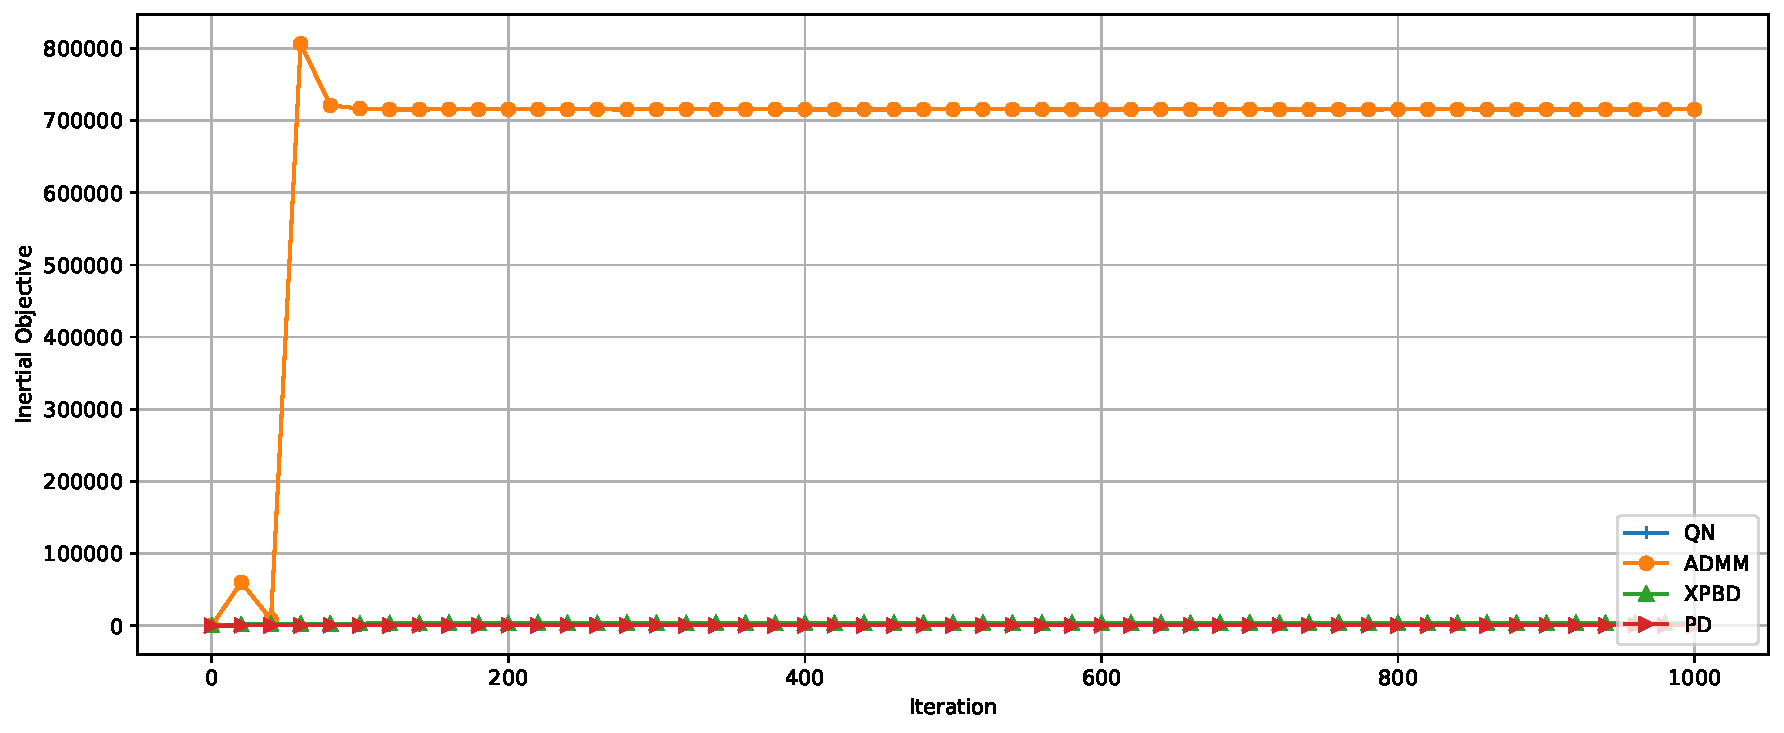
\includegraphics[width=\linewidth]{figures/strain_beam_twist_inertialObjective.pdf}
    \end{subfigure}
    \caption{Values of the constraint (top) and inertial (bottom) terms of the objective function of the variational form of implicit Euler integration 
        (see Eq.\ \ref{eq:variational-implicit}) over the iterations of a single time step of size \SI{1e-1}{\second} for an untwisting beam with strain 
    constraints with stiffness \num{1e9}.}
    \label{fig:strain-beam-twist-objectives-split}
\end{figure}

Again, we create separate plots for the constraint and inertial terms of the objective function in Figure \ref{fig:strain-beam-twist-objectives-split}. The graph for the 
constraint term looks almost identical to the graph for the entire objective function in Figure \ref{fig:strain-beam-twist-objectives}. During the first 40 iterations, the 
constraint term achieved by ADMM is larger than the constraint term that QN and PD converge to. After 80 ADMM iterations, the constraint term converges to a value that is 
significantly lower than the one achieved by the other PD-style solvers. The most dramatic decrease in the constraint term occurs between 40 and 60 ADMM iterations. At the 
same time, ADMM's inertial term increases dramatically. The final inertial term achieved by ADMM is significantly higher than the inertial terms achieved by all other solvers, 
including XPBD.

The results suggest that ADMM is able to find particle positions that yield much lower constraint energies than the other solvers. The fact that the decrease in the 
constraint term between 40 and 60 iterations goes along with a sharp increase in the inertial term indicates that these particle positions differ significantly from the 
initial twisted configuration. This is surprising, since the reference positions of the position constraints at the ends of the beam that initiate the twisting motion 
are only rotated by a couple of degrees. Thus, we would expect the optimal configuration to have a small inertial term, as is observed for the configurations that 
QN and PD converge to. One possible explanation is that QN and PD converge to a local minimum of the objective function, whereas ADMM converges to a global solution. This 
hypothesis is supported by the observation that ADMM increases the objective value during the first 20 iterations (see Fig. \ref{fig:strain-beam-twist-objectives}). Informally, this 
suggests that the ADMM solver spends the early solver iterations escaping the valley containing the local minimum that QN and PD converge to so that the global minimum 
can be achieved during later iterations.

\begin{figure}
    \begin{subfigure}{0.49\textwidth}
    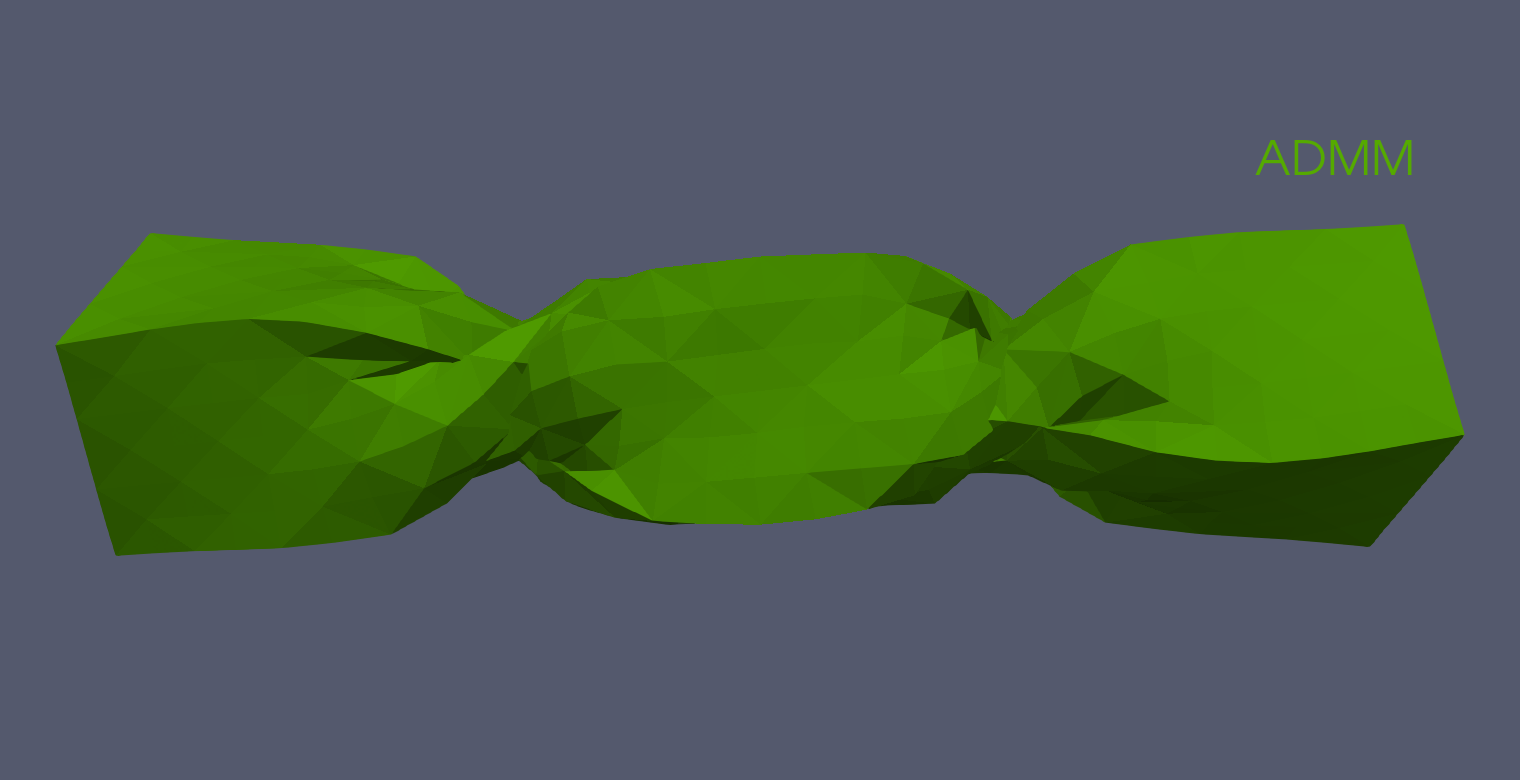
\includegraphics[width=\textwidth, trim={0 5.0cm 0 2.5cm}, clip]{figures/twisted_beam_bad_state_admm.png}
    \subcaption{20 iterations ADMM}
    \end{subfigure}
    \begin{subfigure}{0.49\textwidth}
    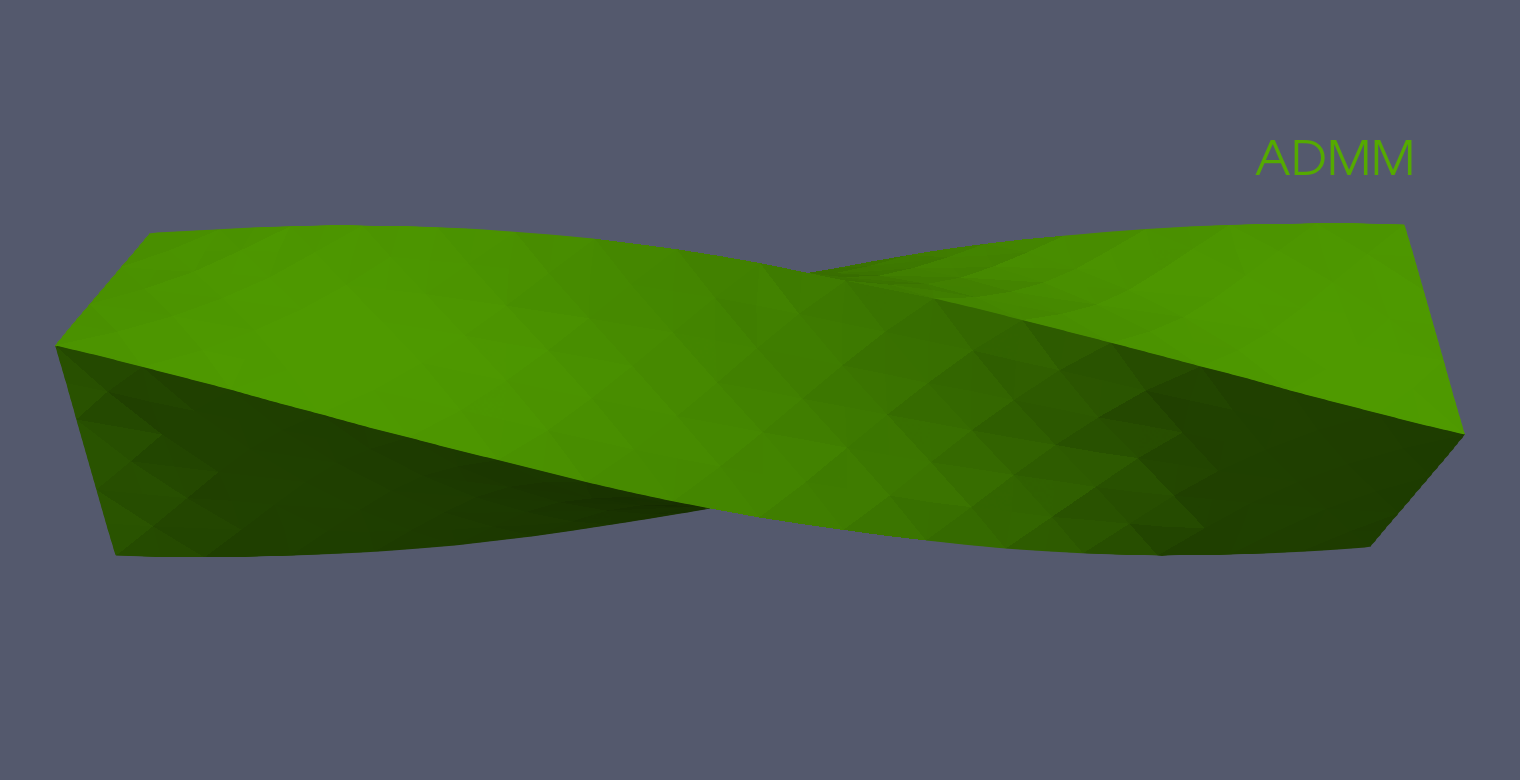
\includegraphics[width=\textwidth, trim={0 5.0cm 0 2.5cm}, clip]{figures/twisted_beam_artificial_state_admm.png}
    \subcaption{1000 iterations ADMM}
    \end{subfigure}
    \centering
    \par\medskip
    \begin{subfigure}{0.49\textwidth}
    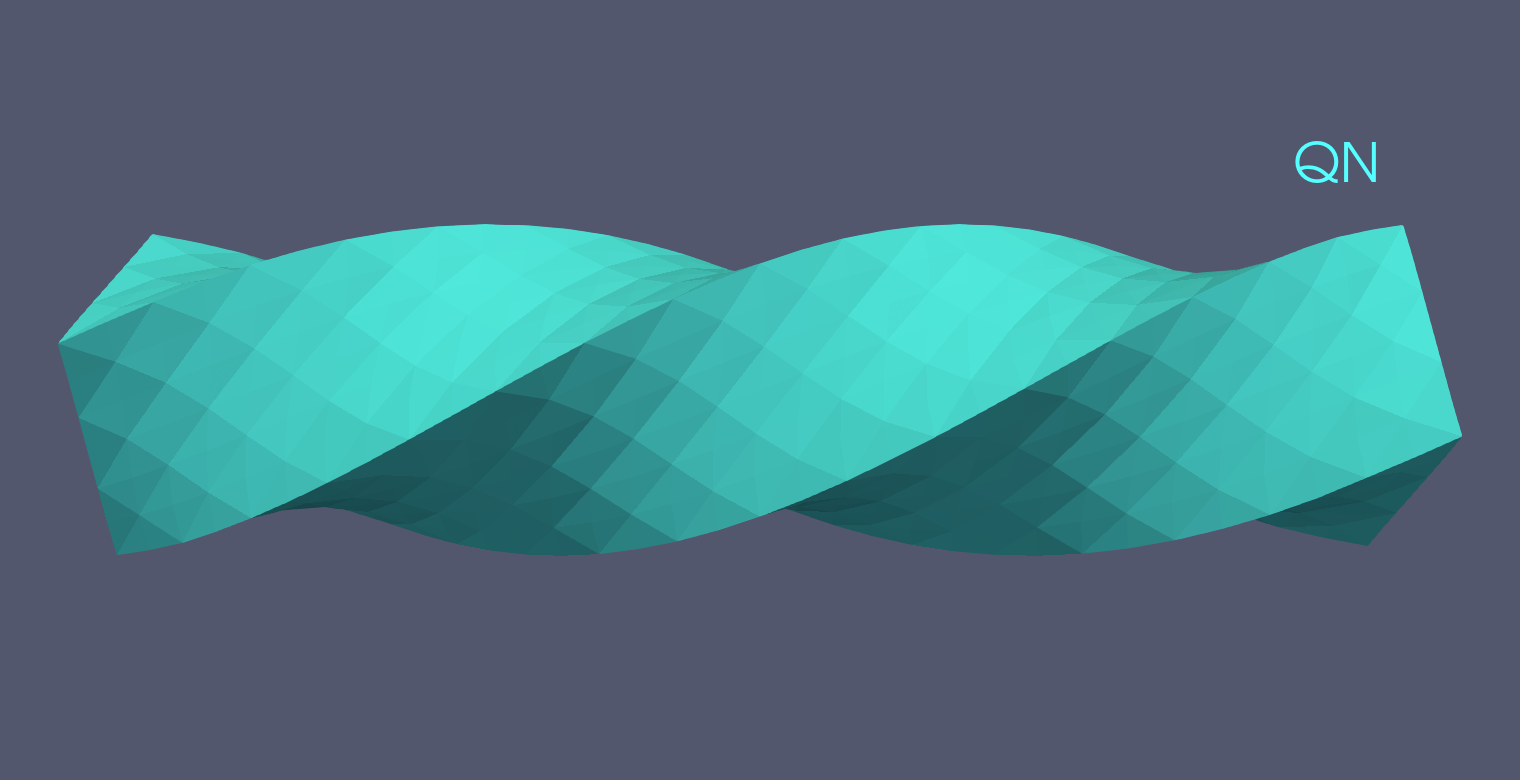
\includegraphics[width=\textwidth, trim={0 5.0cm 0 2.5cm}, clip]{figures/twisted_beam_qn.png}
    \subcaption{QN after convergence}
    \end{subfigure}
    \caption{Geometries of a twisting beam with strain constraints (stiffness \num{1e10}) after 20 (a) and 1000 (b) ADMM iterations over a time step of size 
        \SI{1e-2}{\second}. The converged QN geometry (c) is given as a reference.}
    \label{fig:strain-beam-twist-admm-geometries}
\end{figure}

To gain more insights, we take a closer look at the ADMM geometries after 20 and 1000 iterations in Figure \ref{fig:strain-beam-twist-admm-geometries}. After 20 ADMM iterations, 
the beam appears overtwisted at two locations at roughly one third and two thirds of the beam width. In the vicinity of these overtwisted locations, the surface of the 
beam is highly irregular. In contrast, the surface of the beam appears smooth at the converged ADMM geometry. At the configuration ADMM converges to, the beam is 
significantly closer to its reference configuration than at the geometry computed by the QN solver. Additionally, the converged ADMM and QN geometries are twisted in 
opposite directions.

The results in Figure \ref{fig:strain-beam-twist-admm-geometries} support the hypothesis that ADMM converges to a global minimum of the objective function, whereas QN and PD 
converge to a local minimum. By overtwisting the beam at two locations, the ADMM solver is eventually able to arrive at a configuration where most of the twist from the 
initial deformed configuration is removed without violating the position constraints at the end of the beam. Recall that the value of the objective function can be 
interpreted as the energy of the beam at a configuration (see Sec.\ \ref{ss:analysis-solvers}). Then, it is obvious that the overtwisting motion required to achieve this 
global minimum is not phyiscally plausible, since the energy of the beam is increased to a larger value than the energy at the initial deformed state in the process.
However, without external forces, the energy of the beam should be conserved according to Newton's laws of motion. For the experiments above, ADMM weights of 
$w_i = 0.3\sqrt{k}$ were used, where $k$ is the strain constraint stiffness. The fact that PD does not converge to the global minimum even though it is almost 
identical to ADMM with weights $w_i = \sqrt{k}$ is in line with our observation that lower ADMM weights encourage more aggressive optimization of the constraint 
energies (see Sec.\ \ref{ss:admm-weights}). Finally, Figure \ref{fig:strain-beam-twist-objectives} and Figure \ref{fig:strain-beam-twist-admm-geometries} highlight the ramifications
of terminating the ADMM solver before convergence is achieved: Early termination can increase the beam energy and cause visual geometric artifacts on the surface of the beam.

\begin{table}[h]
\centering
\begin{tabular}{ |r||c|c|c|c| } 
     \hline
     time step in s & \num{1e-1} & \num{1e-2} & \num{1e-3} & \num{1e-4}\\ 
     \hline
     stiffness & \num{1e6} & \num{1e10} & \num{1e10} & \num{1e12} \\
     & \num{1e8}  &  &  \num{1e12} &  \\
     & \num{1e11} &  &  &\\
     \hline
    \end{tabular}
\caption{Combinations of time step sizes and stiffness values for which the ADMM solver converges to the global minimum during the twisting beam experiments using 
the strain material model.}
\label{fig:strain-beam-twist-admm-artificial}
\end{table}

For each time step size, we list the stiffness values for which ADMM converges to the global minimum in the twisting beam experiments in 
Figure \ref{fig:strain-beam-twist-admm-artificial}. For the large time step \SI{1e-1}{\second}, the ADMM solver converges to the global minimum for stiffness values as 
low as \num{1e6}. As the time step size is decreased, larger stiffness values are required. Since achieving the global minimum requires moving particles far away 
from their inertial positions, it is expected that such aggressive minimizations of the constraint energies are favored by large stiffness values and large time steps
(see Sec.\ \ref{ss:variational-implicit-euler}). Still, it is likely that the choice of the ADMM weights has a strong impact on whether the ADMM solver converges to the 
the global minimum or not.

Lastly, we show that there are time step sizes and stiffness values for which ADMM does not converge at all in the twisting beam scenario. Conside the plot of the 
objective values over the iterations for a time step of \SI{1e-2}{\second} and a stiffness value of \num{1e8} in 
Figure \ref{fig:strain-beam-twist-objectives-admm-failure}. The graphs show that ADMM oscillates between configurations with objective values that are larger 
than the initial objective value and objective values that are smaller than the minimal objective values achieved by QN and PD. Similar results are observed for 
time step size \SI{1e-1}{\second} and stiffness \num{1e10} and timestep size \SI{1e-2} and stiffness values \num{1e8} and \num{1e10}.

\begin{figure}[h]
    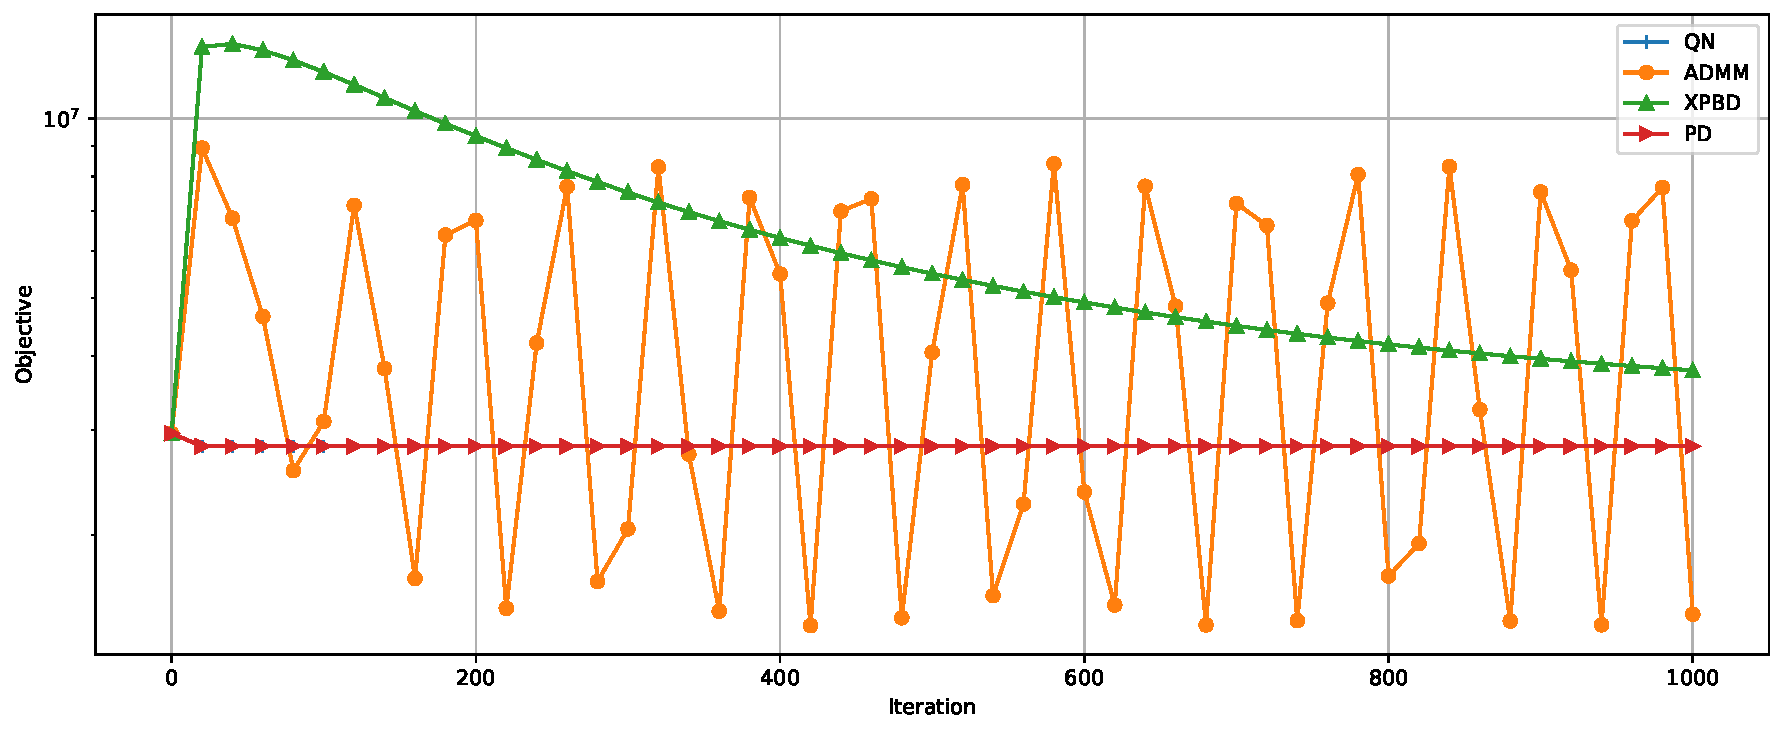
\includegraphics[width=\textwidth]{figures/strain_beam_twist_objectives_admm_failure.pdf}
    \caption{Values of the objective function of the variational form of implicit Euler integration (see Eq.\ \ref{eq:variational-implicit}) over the iterations of 
        a single time step of size \SI{1e-2}{\second} for a twisting beam using strain constraints with stiffness \num{1e8}.}
    \label{fig:strain-beam-twist-objectives-admm-failure}
\end{figure}

Together with the results discussed above, the data from Figure \ref{fig:strain-beam-twist-objectives-admm-failure} suggests that ADMM drives particle 
positions towards the global minimum of the objective function, but eventually undoes its progress once the particle positions get too close. It is not clear why 
this failure to converge occurs for the parameters listed above, but not for the parameters in Figure \ref{fig:strain-beam-twist-admm-artificial}. Again, the choice 
of the ADMM weights most likely plays an important role here. Recall that ADMM weights used during the twisting beam experiments were adopted from the corresponding 
parameter screens for the untwisting beam experiments (see Sec.\ \ref{ss:admm-weights}). In light of the similarities between PD and ADMM with weights $w_i = \sqrt{k}$, 
it is reasonable to assume that convergence could be achieved with more appropriate ADMM weights. As a result, it might be necessary to fine-tune ADMM weights for 
individual simulation scenarios. Of course, this is highly impractical.

\section{Untwisting Beam Simulations - Neohookean Material}\label{ss:untwisting-beam-neohookean}

\section{Discussion}\label{s:discussion}

% TODO:
% - ADMM weights for neohookean model
% - XPBD formulations for neohookean model (incompressibility, stability)
% - Iteration times XPBD solvers
